% build using
%    lhs2TeX GuabaoPaper.lhs | pdflatex --jobname=GuabaoPaper

\documentclass[runningheads]{llncs}

%% ODER: format ==         = "\mathrel{==}"
%% ODER: format /=         = "\neq "
%
%
\makeatletter
\@ifundefined{lhs2tex.lhs2tex.sty.read}%
  {\@namedef{lhs2tex.lhs2tex.sty.read}{}%
   \newcommand\SkipToFmtEnd{}%
   \newcommand\EndFmtInput{}%
   \long\def\SkipToFmtEnd#1\EndFmtInput{}%
  }\SkipToFmtEnd

\newcommand\ReadOnlyOnce[1]{\@ifundefined{#1}{\@namedef{#1}{}}\SkipToFmtEnd}
\usepackage{amstext}
\usepackage{amssymb}
\usepackage{stmaryrd}
\DeclareFontFamily{OT1}{cmtex}{}
\DeclareFontShape{OT1}{cmtex}{m}{n}
  {<5><6><7><8>cmtex8
   <9>cmtex9
   <10><10.95><12><14.4><17.28><20.74><24.88>cmtex10}{}
\DeclareFontShape{OT1}{cmtex}{m}{it}
  {<-> ssub * cmtt/m/it}{}
\newcommand{\texfamily}{\fontfamily{cmtex}\selectfont}
\DeclareFontShape{OT1}{cmtt}{bx}{n}
  {<5><6><7><8>cmtt8
   <9>cmbtt9
   <10><10.95><12><14.4><17.28><20.74><24.88>cmbtt10}{}
\DeclareFontShape{OT1}{cmtex}{bx}{n}
  {<-> ssub * cmtt/bx/n}{}
\newcommand{\tex}[1]{\text{\texfamily#1}}	% NEU

\newcommand{\Sp}{\hskip.33334em\relax}


\newcommand{\Conid}[1]{\mathit{#1}}
\newcommand{\Varid}[1]{\mathit{#1}}
\newcommand{\anonymous}{\kern0.06em \vbox{\hrule\@width.5em}}
\newcommand{\plus}{\mathbin{+\!\!\!+}}
\newcommand{\bind}{\mathbin{>\!\!\!>\mkern-6.7mu=}}
\newcommand{\rbind}{\mathbin{=\mkern-6.7mu<\!\!\!<}}% suggested by Neil Mitchell
\newcommand{\sequ}{\mathbin{>\!\!\!>}}
\renewcommand{\leq}{\leqslant}
\renewcommand{\geq}{\geqslant}
\usepackage{polytable}

%mathindent has to be defined
\@ifundefined{mathindent}%
  {\newdimen\mathindent\mathindent\leftmargini}%
  {}%

\def\resethooks{%
  \global\let\SaveRestoreHook\empty
  \global\let\ColumnHook\empty}
\newcommand*{\savecolumns}[1][default]%
  {\g@addto@macro\SaveRestoreHook{\savecolumns[#1]}}
\newcommand*{\restorecolumns}[1][default]%
  {\g@addto@macro\SaveRestoreHook{\restorecolumns[#1]}}
\newcommand*{\aligncolumn}[2]%
  {\g@addto@macro\ColumnHook{\column{#1}{#2}}}

\resethooks

\newcommand{\onelinecommentchars}{\quad-{}- }
\newcommand{\commentbeginchars}{\enskip\{-}
\newcommand{\commentendchars}{-\}\enskip}

\newcommand{\visiblecomments}{%
  \let\onelinecomment=\onelinecommentchars
  \let\commentbegin=\commentbeginchars
  \let\commentend=\commentendchars}

\newcommand{\invisiblecomments}{%
  \let\onelinecomment=\empty
  \let\commentbegin=\empty
  \let\commentend=\empty}

\visiblecomments

\newlength{\blanklineskip}
\setlength{\blanklineskip}{0.66084ex}

\newcommand{\hsindent}[1]{\quad}% default is fixed indentation
\let\hspre\empty
\let\hspost\empty
\newcommand{\NB}{\textbf{NB}}
\newcommand{\Todo}[1]{$\langle$\textbf{To do:}~#1$\rangle$}

\EndFmtInput
\makeatother
%
%
%
% First, let's redefine the forall, and the dot.
%
%
% This is made in such a way that after a forall, the next
% dot will be printed as a period, otherwise the formatting
% of `comp_` is used. By redefining `comp_`, as suitable
% composition operator can be chosen. Similarly, period_
% is used for the period.
%
\ReadOnlyOnce{forall.fmt}%
\makeatletter

% The HaskellResetHook is a list to which things can
% be added that reset the Haskell state to the beginning.
% This is to recover from states where the hacked intelligence
% is not sufficient.

\let\HaskellResetHook\empty
\newcommand*{\AtHaskellReset}[1]{%
  \g@addto@macro\HaskellResetHook{#1}}
\newcommand*{\HaskellReset}{\HaskellResetHook}

\global\let\hsforallread\empty

\newcommand\hsforall{\global\let\hsdot=\hsperiodonce}
\newcommand*\hsperiodonce[2]{#2\global\let\hsdot=\hscompose}
\newcommand*\hscompose[2]{#1}

\AtHaskellReset{\global\let\hsdot=\hscompose}

% In the beginning, we should reset Haskell once.
\HaskellReset

\makeatother
\EndFmtInput
%
%
%
%
%
% This package provides two environments suitable to take the place
% of hscode, called "plainhscode" and "arrayhscode". 
%
% The plain environment surrounds each code block by vertical space,
% and it uses \abovedisplayskip and \belowdisplayskip to get spacing
% similar to formulas. Note that if these dimensions are changed,
% the spacing around displayed math formulas changes as well.
% All code is indented using \leftskip.
%
% Changed 19.08.2004 to reflect changes in colorcode. Should work with
% CodeGroup.sty.
%
\ReadOnlyOnce{polycode.fmt}%
\makeatletter

\newcommand{\hsnewpar}[1]%
  {{\parskip=0pt\parindent=0pt\par\vskip #1\noindent}}

% can be used, for instance, to redefine the code size, by setting the
% command to \small or something alike
\newcommand{\hscodestyle}{}

% The command \sethscode can be used to switch the code formatting
% behaviour by mapping the hscode environment in the subst directive
% to a new LaTeX environment.

\newcommand{\sethscode}[1]%
  {\expandafter\let\expandafter\hscode\csname #1\endcsname
   \expandafter\let\expandafter\endhscode\csname end#1\endcsname}

% "compatibility" mode restores the non-polycode.fmt layout.

\newenvironment{compathscode}%
  {\par\noindent
   \advance\leftskip\mathindent
   \hscodestyle
   \let\\=\@normalcr
   \let\hspre\(\let\hspost\)%
   \pboxed}%
  {\endpboxed\)%
   \par\noindent
   \ignorespacesafterend}

\newcommand{\compaths}{\sethscode{compathscode}}

% "plain" mode is the proposed default.
% It should now work with \centering.
% This required some changes. The old version
% is still available for reference as oldplainhscode.

\newenvironment{plainhscode}%
  {\hsnewpar\abovedisplayskip
   \advance\leftskip\mathindent
   \hscodestyle
   \let\hspre\(\let\hspost\)%
   \pboxed}%
  {\endpboxed%
   \hsnewpar\belowdisplayskip
   \ignorespacesafterend}

\newenvironment{oldplainhscode}%
  {\hsnewpar\abovedisplayskip
   \advance\leftskip\mathindent
   \hscodestyle
   \let\\=\@normalcr
   \(\pboxed}%
  {\endpboxed\)%
   \hsnewpar\belowdisplayskip
   \ignorespacesafterend}

% Here, we make plainhscode the default environment.

\newcommand{\plainhs}{\sethscode{plainhscode}}
\newcommand{\oldplainhs}{\sethscode{oldplainhscode}}
\plainhs

% The arrayhscode is like plain, but makes use of polytable's
% parray environment which disallows page breaks in code blocks.

\newenvironment{arrayhscode}%
  {\hsnewpar\abovedisplayskip
   \advance\leftskip\mathindent
   \hscodestyle
   \let\\=\@normalcr
   \(\parray}%
  {\endparray\)%
   \hsnewpar\belowdisplayskip
   \ignorespacesafterend}

\newcommand{\arrayhs}{\sethscode{arrayhscode}}

% The mathhscode environment also makes use of polytable's parray 
% environment. It is supposed to be used only inside math mode 
% (I used it to typeset the type rules in my thesis).

\newenvironment{mathhscode}%
  {\parray}{\endparray}

\newcommand{\mathhs}{\sethscode{mathhscode}}

% texths is similar to mathhs, but works in text mode.

\newenvironment{texthscode}%
  {\(\parray}{\endparray\)}

\newcommand{\texths}{\sethscode{texthscode}}

% The framed environment places code in a framed box.

\def\codeframewidth{\arrayrulewidth}
\RequirePackage{calc}

\newenvironment{framedhscode}%
  {\parskip=\abovedisplayskip\par\noindent
   \hscodestyle
   \arrayrulewidth=\codeframewidth
   \tabular{@{}|p{\linewidth-2\arraycolsep-2\arrayrulewidth-2pt}|@{}}%
   \hline\framedhslinecorrect\\{-1.5ex}%
   \let\endoflinesave=\\
   \let\\=\@normalcr
   \(\pboxed}%
  {\endpboxed\)%
   \framedhslinecorrect\endoflinesave{.5ex}\hline
   \endtabular
   \parskip=\belowdisplayskip\par\noindent
   \ignorespacesafterend}

\newcommand{\framedhslinecorrect}[2]%
  {#1[#2]}

\newcommand{\framedhs}{\sethscode{framedhscode}}

% The inlinehscode environment is an experimental environment
% that can be used to typeset displayed code inline.

\newenvironment{inlinehscode}%
  {\(\def\column##1##2{}%
   \let\>\undefined\let\<\undefined\let\\\undefined
   \newcommand\>[1][]{}\newcommand\<[1][]{}\newcommand\\[1][]{}%
   \def\fromto##1##2##3{##3}%
   \def\nextline{}}{\) }%

\newcommand{\inlinehs}{\sethscode{inlinehscode}}

% The joincode environment is a separate environment that
% can be used to surround and thereby connect multiple code
% blocks.

\newenvironment{joincode}%
  {\let\orighscode=\hscode
   \let\origendhscode=\endhscode
   \def\endhscode{\def\hscode{\endgroup\def\@currenvir{hscode}\\}\begingroup}
   %\let\SaveRestoreHook=\empty
   %\let\ColumnHook=\empty
   %\let\resethooks=\empty
   \orighscode\def\hscode{\endgroup\def\@currenvir{hscode}}}%
  {\origendhscode
   \global\let\hscode=\orighscode
   \global\let\endhscode=\origendhscode}%

\makeatother
\EndFmtInput
%

\ReadOnlyOnce{Formatting.fmt}%
\makeatletter

\let\Varid\mathit
\let\Conid\mathit
%%subst keyword a        = "\keyw{" a "}"
%%subst numeral a        = "\con{" a "}"
%%subst string  a        = "\con{\text{\tt \char34 " a "\char34}}"
%%subst char    a        = "\con{\text{\tt ''" a "''}}"

%%\colorlet{identifier}{blue!45!black}
%%\colorlet{constructor}{green!45!black}
%%\colorlet{keyword}{red!40!black}
%%\colorlet{darkgreen}{green!30!black}

%%\newcommand{\keyw}[1]{{\color{keyword}\textsf{\textbf{#1}}}}
\newcommand{\ty}[1]{\Conid{#1}}
\newcommand{\con}[1]{\Conid{#1}}
\newcommand{\id}[1]{\Varid{#1}}
\newcommand{\cl}[1]{\Varid{#1}}
\newcommand{\opsym}[1]{\mathrel{#1}}

\newcommand\Keyword[1]{\textbf{\textsf{#1}}}
\newcommand\Hide{\mathbin{\downarrow}}
\newcommand\Reveal{\mathbin{\uparrow}}



%%format <=> = "\mathrel{\Leftrightarrow}"



\def\commentbegin{\quad\{\ }
\def\commentend{\}}

\makeatother
\EndFmtInput


%%format (assert (x)) = "\{" x "\}"
   %% using \assert in macros.tex for coloring.

%% Array








 %\newcommand{\lBracP}{\lbrack\!\{}
 % \newcommand{\rBracP}{\}\!\rbrack}
\newcommand{\lBracP}{(\!\lbrack}
\newcommand{\rBracP}{\rbrack\!)}
 % \newcommand{\lBracP}{(\!\!\{}
 % \newcommand{\rBracP}{\}\!\!)}

%%format (subst (x) (e)) = "\subst{" x "}{" e "}"



\newcommand{\veryshortarrow}[1][3pt]{\mathrel{%
   \hbox{\rule[\dimexpr\fontdimen22\textfont2-.2pt\relax]{#1}{.4pt}}%
   \mkern-4mu\hbox{\usefont{U}{lasy}{m}{n}\symbol{41}}}}

%%format funalt f (i) (e) = f "\lbrack" i "\veryshortarrow" e "\rbrack"
%%format funalt f (i) (e) = f "\lbrack" i "\rightharpoonup" e "\rbrack"
%%format funalt f (i) (e) = f "\lbrack" i ":" e "\rbrack"


%% Pointers

\newcommand{\shortmapsto}{\hstretch{0.6}{\mapsto}}
\newcommand{\shookrarrow}{\hstretch{0.6}{\hookrightarrow}}







%
%
%
%
\ReadOnlyOnce{lineno.fmt}%
\makeatletter

\newcounter{linenum}
\newcounter{linestep}
\newlength{\linetemp}% ugly, remove the need for a dimen register

\newcommand{\linenumsetupleft}{\column{line}{@{}l@{}}\column{lineend}{}\column{B}{}}
%\newcommand{\linenumsetupleft}{\column{line}{@@{}>{\setbox0=\hbox\bgroup}l<{\egroup\makebox[0pt][r]{\box0\ }}@@{}}\column{lineend}{}\column{B}{}}
\newcommand{\linenumsetupright}{\setlength{\linetemp}{\linewidth-\mathindent}\column[\linetemp]{line}{@{}l@{}}\column{lineend}{}\column{B}{}}
\newcommand{\linenumfromtoleft}{\refstepcounter{linenum}\fromto{line}{lineend}}
\newcommand{\linenumfromtoright}{\refstepcounter{linenum}\fromto{line}{lineend}}
\newcommand{\numbersright}{\let\linenumsetup\linenumsetupright\let\printlinebegin\empty\def\printlineend{\printline}\let\linenumfromto\linenumfromtoright\def\linenumalign{l}}
\newcommand{\numbersleft}{\let\linenumsetup\linenumsetupleft\def\printlinebegin{\printline}\let\printlineend\empty\let\linenumfromto\linenumfromtoleft\def\linenumalign{r}}
\numbersleft
\newcommand{\printlineyes}{%
  \linenumfromto{%
    \stepcounter{linestep}%
    \ifthenelse{\value{linestep}<\linenumstep}{}{%
      \formatlinenum{\thelinenum}%
      \setcounter{linestep}{0}}}}
\newcommand*{\formatlinenum}[1]{\makebox[\linenumwidth][\linenumalign]{\ \,{\footnotesize #1}\ \,}}
\newcommand*{\numberwidth}[1]{\def\linenumwidth{#1}}
\numberwidth{0pt}
\newcommand*{\numberstep}[1]{\def\linenumstep{#1}}
\numberstep{1}
\newcommand{\numberson}{\global\let\printline\printlineyes}
\newcommand{\numbersoff}{\global\let\printline\empty}
\newcommand{\numbersreset}{\setcounter{linenum}{0}}
\numberson
%

\usepackage[T1]{fontenc}
\usepackage{graphicx}

\usepackage{amsfonts}
\usepackage{amsmath}
\usepackage{scalerel}
\usepackage{hyperref}
\usepackage{url}
\usepackage{xcolor}
\usepackage{textcomp}
\usepackage{paralist}
\usepackage{caption}
\usepackage{subcaption}
\usepackage{CJKutf8}
\newcommand{\cjk}[1]{\begin{CJK*}{UTF8}{bsmi}{\small #1}\end{CJK*}}
\usepackage{adjustbox}
\usepackage{ifthen}

\newcommand{\delete}[1]{}
\newcommand{\assert}[1]{\{ #1 \}}

\newcommand{\htriple}[3]{\assert{#1}\,#2\,\assert{#3}}
\newcommand{\htripletwo}[5]{\assert{#1}\,#2\,\assert{#3}\,#4\,\assert{#5}}

\makeatletter
\@ifpackageloaded{stix}{%
}{%
  \DeclareFontEncoding{LS2}{}{\noaccents@}
  \DeclareFontSubstitution{LS2}{stix}{m}{n}
  \DeclareSymbolFont{stix@largesymbols}{LS2}{stixex}{m}{n}
  \SetSymbolFont{stix@largesymbols}{bold}{LS2}{stixex}{b}{n}
  \DeclareMathDelimiter{\lBrace}{\mathopen} {stix@largesymbols}{"E8}%
                                            {stix@largesymbols}{"0E}
  \DeclareMathDelimiter{\rBrace}{\mathclose}{stix@largesymbols}{"E9}%
                                            {stix@largesymbols}{"0F}
}
\makeatother


\renewcommand*{\formatlinenum}[1]{\makebox[3em][l]{\scriptsize{#1}}}%

\numbersoff

\newcommand{\todo}[1]{{\bf Todo}: \lbrack #1 \rbrack}

\newcommand{\sshotimg}[1]{
\adjustbox{padding*=2ex 8ex 2ex 8ex, max width=\textwidth}{%
\includegraphics{img/#1.jpg}}}

\begin{document}

\title{Imperative Program Derivation in Guabao
%\thanks{Supported by organization x.}
}

\author{Shin-Cheng Mu\inst{1}%\orcidID{0000-0002-4755-601X}
\and
Ting-Yan Lai\inst{1}\and
Thing-Han Lim\inst{1}\and
Chien-Yuan Su\inst{1}\and
Hsien-En Tzeng\inst{2}%
}
%
\authorrunning{S-C. Mu  et al.}

\institute{
%Institute of Information Science, %\\
Academia Sinica, Taiwan \and
National Taiwan University, Taiwan
}


\maketitle              % typeset the header of the contribution
%
\begin{abstract}
Guabao is an integrated environment for imperative program derivation --- the process of formally and step-wise constructing a program from its specification.
As the programmer types in the code, in a variation of Guarded Command Language,
Guabao computes its proof obligations in an interface that encourages the program and its correctness proof to be developed hand in hand.
We present the user experience of Guabao, the algorithm it uses to compute proof obligations and infer pre/postconditions, and compare it with contemporary tools serving similar purposes.
\keywords{program derivation \and integrated developing environment \and proofs}
\end{abstract}

\section{Introduction}

\begin{quote}
\ldots to prove the correctness of a given program was in a sense putting the cart before the horse. A much more promising approach turned out to be letting correctness proof and program grow hand in hand: with the choice of the structure of the correctness proof one designs a program for which this proof is applicable. The fact that then the correctness concerns turn out to act as an inspiring heuristic guidance is an added benefit.
\begin{flushright}
--- E. W. Dijkstra, 1973. \cite{Dijkstra:74:Programming}
\end{flushright}
\end{quote}

\emph{Program derivation} is the process of formally and step-wise constructing a program from its specification, such that every step is mathematically justifiable. As a methodology to construct reliable software, its central idea is that, rather than verifying a program after it has been written, \emph{a program and its correctness proof should be developed hand in hand}.
This does not necessarily imply more work for the programmer.
On the contrary, as argued in the quote above, thinking about how a program can be proven correct often gives useful hints on how to construct the program.

Theories of imperative program derivation based on the \emph{weakest precondition} calculus was initially developed by Dijkstra~\cite{Dijkstra:75:Guarded}.
It can be seen as a variation of Hoare logic~\cite{Hoare:69:Axiomatic} where, instead of a more conventional operational semantics, the meaning of a program is taken to be a \emph{predicate transformer}: a function that, given a desired postcondition $Q$, yields the weakest precondition $P$ such that the program will terminate in a state that satisfies $Q$.
This view of programs invites the programmer to abstract away from how the program operationally carries out its task, and instead to focus on the postcondition that the programmer wants to achieve.
The program is then derived by manipulating the pre/postconditions using various calculational rules.
Various previous work~\cite{Dijkstra:76:Discipline,%
Gries:81:Science,Kaldewaij:90:Programming,Morgan:90:Programming,%
Backhouse:03:Program,Backhouse:11:Algorithmic} collectively developed a methodology of program development from specification, equipped with techniques for constructing a loop invariant from a desired postcondition, constructing the loop body from its last step, ensuring termination, etc.
This methodology was applied to derive algorithms
solving individual small problems
(e.g~\cite{Rem:89:Small,Rem:90:Small}) as well as families of problems (e.g~\cite{Zantema:92:Longest}).
% Meanwhile, derivation of functional programs, a closely related topic, has also been developing (e.g~\cite{Bird:10:Pearls}).
Within the advocating community it is at least wished that the concept of program derivation should be taught as part of the fundamental training for programmers and computing science majors.
% These days, program derivation is more practiced in the functional programming community. Derivation of imperative programs, however, is also a field with rich possibilities and potentials.

Since 2011, the first author has been teaching an undergraduate level Programming Languages course, in which imperative program derivation is covered.
From the experiences accumulated, we felt that such a course would benefit from having a supporting tool.
Therefore we created Guabao.
The aim is to develop a programming environment having the following features:
\begin{enumerate}
\item It encourages {\bf developing proofs and programs together}.
While the user may certainly write up all the code in Guabao and verify it afterwards, the interface shall allow the user to interleave proving and coding, and let the two modes aid each other.
\item It encourages {\bf backward-reasoning}.
Since it is easier to construct the weakest precondition of an assignment (\ensuremath{\Varid{x}\mathbin{:=}\Varid{e}}) from its postcondition than the other way round,
to construct a block of statements, many derivation techniques start with thinking about what the \emph{last assignment} could be.
The interface of Guabao should make such construction easy and natural.
\item It allows {\bf free-form text editing}, as opposed to treating programs as diagrams as some program construction tools do, since we believe it what most programmers would prefer.
\end{enumerate}
In Section~\ref{sec:programming-example} we will see an example demonstrating all these features.
It might also help to clarify what Guabao is not:
\begin{enumerate}
\item Gaubao is not an implementation of Guarded Command Language (GCL).
Dijkstra~\cite{Dijkstra:98:Cruelty} wrote that he would
design a programming language for teaching (which we believe would be GCL) and ``see to it that [it] has not been implemented on campus so that students are protected from the temptation to test their programs.''
Gaubao is not an implementation of GCL in which one can write a program and test it, but an environment where a program and its proof can be designed together.
% One cannot yet execute the program --- although it is not difficult to implement an interpreter and allow a program to run once all proofs are done.
\item Guabao does not intend to prove \emph{everything} regard the correctness of the program for the user.
Instead, it computes the proof obligations needed to guarantee correctness, and let them guide the development of the said program.
Guabao does employ an SMT solver (currently Z3~\cite{MS:12:Z3}) to discharge simple proof obligations.
However, we believe that proving properties that are related to the algorithmic aspect of a program and, in case of failure, learning from the proof how the program should evolve to allow the proof to go through, is a part of the program development process, which should be carried out by the user.
It is especially so in a course teaching program derivation.
Currently Guabao does not check user-written proofs.
To do so we shall develop a representation of equational proofs, which is one of our future works.
\end{enumerate}

Guabao is implemented as an extension of the editor Visual Studio Code,
which can be installed by searching for the extension "Guabao" in the editor, or through its Extensions Marketplace~\footnote{\url{https://marketplace.visualstudio.com/items?itemName=scmlab.guabao}}.
A simple one-click installation downloads the frontend and the pre-compiled backend.%
~\footnote{Z3 has to be installed separately, however.}
%The readers are welcomed to give it a try!
The backend of Guabao is implemented using Haskell~\cite{PeytonJones:03:Haskell}, while the frontend is implemented using Reason~\cite{Walke:16:Reason} and compiled to Javascript to run in VS Code.
Regarding its name,
GUA in Guabao comes from GUArded command language.
Guabao (\cjk{刈包}) is a street food popular in places including Taiwan, where Guabao the software was designed.

After giving a brief review of the Guarded Command Language in Section~\ref{sec:gcl}, we demonstrate how it is like using Guabao by a simple example in Section~\ref{sec:programming-example}.
Section~\ref{sec:po-generation} presents the algorithm we use to generate proof obligations and infer pre/postconditions of specs.
We compare Guabao with some other tools in Section~\ref{sec:related-works}
before we conclude in Section~\ref{sec:conclude}.

\section{The Guarded Command Language}
\label{sec:gcl}

\begin{figure}[t]
\begin{hscode}\linenumsetup\printlinebegin\SaveRestoreHook
\column{B}{@{}>{\hspre}l<{\hspost}@{}}%
\column{8}{@{}>{\hspre}c<{\hspost}@{}}%
\column{8E}{@{}l@{}}%
\column{13}{@{}>{\hspre}l<{\hspost}@{}}%
\column{E}{@{}>{\hspre}l<{\hspost}@{}}%
\>[B]{}\Conid{Prog}{}\<[8]%
\>[8]{}\mathbin{::=}{}\<[8E]%
\>[13]{}{\Conid{Decl}}^{*}\;{\Conid{Stmt}}^{*}{}\<[E]%
\printlineend\\
\printlinebegin\>[B]{}\Conid{Decl}{}\<[8]%
\>[8]{}\mathbin{::=}{}\<[8E]%
\>[13]{}\mathbf{var}\;{\Conid{Var}}^{+}\mathbin{:}\Conid{Type}\mathbin{?}\!\assert{\Conid{Expr}}\mid \mathbf{con}\;{\Conid{Var}}^{+}\mathbin{:}\Conid{Type}\mathbin{?}\!\assert{\Conid{Expr}}{}\<[E]%
\printlineend\\
\printlinebegin\>[B]{}\Conid{Stmt}{}\<[8]%
\>[8]{}\mathbin{::=}{}\<[8E]%
\>[13]{}\assert{\Conid{Expr}}\mid \Varid{skip}\mid \Varid{abort}\mid {\Conid{Var}}^{+}\mathbin{:=}{\Conid{Expr}}^{+}{}\<[E]%
\printlineend\\
\printlinebegin\>[8]{}\mid {}\<[8E]%
\>[13]{}\mathbf{do}\;{\Conid{GdCmd}}^{*}\;\mathbf{od}\mid \mathbf{if}\;{\Conid{GdCmd}}^{*}\;\mathbf{fi}{}\<[E]%
\printlineend\\
\printlinebegin\>[B]{}\Conid{GdCmd}{}\<[8]%
\>[8]{}\mathbin{::=}{}\<[8E]%
\>[13]{}\Conid{Expr}\to {\Conid{Stmt}}^{+}{}\<[E]%
\printlineend\ColumnHook
\end{hscode}\resethooks
\caption{An abstract syntax of Guarded Command Language.
\ensuremath{\Conid{Var}} denotes the collection of variable identifiers.
Definitions of \ensuremath{\Conid{Expr}} and \ensuremath{\Conid{Type}} are omitted.}
\label{fig:gcl-syntax}
\end{figure}

Guabao uses a variation of the Guarded Command Language (GCL)~\cite{Dijkstra:75:Guarded},
which we will briefly review in this section,
emphasising on what needs to be proved about a given statement.
A condensed presentation of its abstract syntax is given in Figure~\ref{fig:gcl-syntax}.
A program consists of a section of declarations followed by a section of statements.
Constant and variable declarations respectively start with keywords \ensuremath{\mathbf{var}} and \ensuremath{\mathbf{con}}.
They can be accompanied by an optional assertion stating properties we assume about the declared entities.

An assertion is a Boolean-valued expression in curly brackets.
By the convention of the program derivation community, a \emph{Hoare triple} \ensuremath{\htriple{\Conid{P}}{\Conid{S}}{\Conid{Q}}} denotes total correctness: that is, the program \ensuremath{\Conid{S}}, when executed in a state satisfying \ensuremath{\Conid{P}}, \emph{terminates} in a state satisfying \ensuremath{\Conid{Q}}.
We prefer it than the partial correctness interpretation (that is, \ensuremath{\Conid{S}} establishes \ensuremath{\Conid{Q}} \emph{if} it terminates) because, as we will see in Section~\ref{sec:programming-example}, that the program must terminate provides useful hints about how it can be written.
% The notation |[!pre, post!]| denotes a \emph{spec} --- a hole yet to be filled in with code that shall establish the postcondition |post| provided that precondition |pre| is satisfied.

% For example, the following is an unfinished program that, upon exit, stores the value of |A * B| in |r|, provided that both |A| and |B| are non-negative.
% \begin{spec}
% CON A, B : Int (assert (A >= 0 && B >= 0))
% VAR r : Int
%
% [: A >= 0 && B >= 0, r = A * B :]
% \end{spec}

The statement \ensuremath{\Varid{skip}} does nothing, while \ensuremath{\Varid{abort}} simply aborts the program.
The operator \ensuremath{\mathbin{:=}} denotes assignment; parallel assignment of multiple variables is allowed.
A \emph{guarded command} \ensuremath{\Conid{B}\to \Conid{S}}, where \ensuremath{\Conid{B}} is a Boolean-valued expression, denotes a command where \ensuremath{\Conid{S}} is executed only if the \emph{guard} \ensuremath{\Conid{B}} evaluates to \ensuremath{\Conid{True}}.

Guarded commands alone do not form a complete statement.
The statement \ensuremath{\mathbf{if}\mathbin{...}\mathbf{fi}}, enclosing a group of guarded commands, denotes conditional branches.
For example, \ensuremath{\mathbf{if}\;\Conid{B}_{0}\to \Conid{S}_{0}\mid \Conid{B}_{1}\to \Conid{S}_{1}\;\mathbf{fi}} has two branches, where \ensuremath{\Conid{S}_{i}} is executed if \ensuremath{\Conid{B}_{i}} holds (\ensuremath{\Varid{i}\in \{\mskip1.5mu \mathrm{0},\mathrm{1}\mskip1.5mu\}}).
If both \ensuremath{\Conid{B}_{0}} and \ensuremath{\Conid{B}_{1}} holds, \emph{one} of the branches is nondeterministically executed.
If neither holds, the program aborts.
To prove that
\begin{hscode}\linenumsetup\printlinebegin\SaveRestoreHook
\column{B}{@{}>{\hspre}l<{\hspost}@{}}%
\column{E}{@{}>{\hspre}l<{\hspost}@{}}%
\>[B]{}\htriple{\Conid{P}}{\mathbf{if}\;\Conid{B}_{0}\to \Conid{S}_{0}\mid \Conid{B}_{1}\to \Conid{S}_{1}\;\mathbf{fi}}{\Conid{Q}}~~,{}\<[E]%
\printlineend\ColumnHook
\end{hscode}\resethooks
one has to prove that 1. \ensuremath{\htriple{\Conid{P}\mathrel{\wedge}\Conid{Bi}}{\Conid{Si}}{\Conid{Q}}} for \ensuremath{\Varid{i}\in \{\mskip1.5mu \mathrm{0},\mathrm{1}\mskip1.5mu\}} --- both branches establish \ensuremath{\Conid{Q}} if executed, and 2. that \ensuremath{\Conid{P}\mathrel{\Rightarrow}\Conid{B}_{0}\mathrel{\vee}\Conid{B}_{1}} --- such that the program would not abort.

A group of guarded commands surrounded by \ensuremath{\mathbf{do}\mathbin{...}\mathbf{od}} denote a while-loop.
In \ensuremath{\mathbf{do}\;\Conid{B}_{0}\to \Conid{S}_{0}\mid \Conid{B}_{1}\to \Conid{S}_{1}\;\mathbf{od}}, for example, when either \ensuremath{\Conid{B}_{0}} or \ensuremath{\Conid{B}_{1}} holds, the corresponding statement \ensuremath{\Conid{S}_{0}} or \ensuremath{\Conid{S}_{1}} gets executed, before we attempt at the next iteration. When neither holds, the loop exits.
In our methodology of program construction,
each loop must have an \emph{invariant} --- a property that shall always hold at the beginning of the loop, and a \emph{bound} --- a value that strictly decreases after each iteration of the loop.
This is denoted by
\begin{hscode}\linenumsetup\printlinebegin\SaveRestoreHook
\column{B}{@{}>{\hspre}l<{\hspost}@{}}%
\column{E}{@{}>{\hspre}l<{\hspost}@{}}%
\>[B]{}\htriple{\Conid{P},\mathbf{bnd}\mathbin{:}\Varid{e}}{\mathbf{do}\;\Conid{B}_{0}\to \Conid{S}_{0}\mid \Conid{B}_{1}\to \Conid{S}_{1}\;\mathbf{od}}{\Conid{Q}}{}\<[E]%
\printlineend\ColumnHook
\end{hscode}\resethooks
where \ensuremath{\Conid{P}} is the loop invariant, \ensuremath{\Varid{e}} the bound, and \ensuremath{\Conid{Q}} the postcondition.

Once we introduce such a loop, however, we have also given ourselves \emph{four} proof obligations:
\begin{hscode}\linenumsetup\printlinebegin\SaveRestoreHook
\column{B}{@{}>{\hspre}l<{\hspost}@{}}%
\column{38}{@{}>{\hspre}l<{\hspost}@{}}%
\column{E}{@{}>{\hspre}l<{\hspost}@{}}%
\>[B]{}\mbox{1. \sf InvBase}:\qquad{}\<[38]%
\>[38]{}\Conid{P}\mathrel{\wedge}\neg \;(\Conid{B}_{0}\mathrel{\vee}\Conid{B}_{1})\mathrel{\Rightarrow}\Conid{Q}~~,{}\<[E]%
\printlineend\\
\printlinebegin\>[B]{}\mbox{2. \sf InvInd}:\qquad{}\<[38]%
\>[38]{}\htriple{\Conid{P}\mathrel{\wedge}\Conid{Bi}}{\Conid{Si}}{\Conid{P}}\;\mbox{,~~for~}\Varid{i}\in \{\mskip1.5mu \mathrm{0},\mathrm{1}\mskip1.5mu\}~~,{}\<[E]%
\printlineend\\
\printlinebegin\>[B]{}\mbox{3. \sf TermBase}:\qquad{}\<[38]%
\>[38]{}\Conid{P}\mathrel{\wedge}(\Conid{B}_{0}\mathrel{\vee}\Conid{B}_{1})\mathrel{\Rightarrow}\Varid{e}\geq \mathrm{0}~~,{}\<[E]%
\printlineend\\
\printlinebegin\>[B]{}\mbox{4. \sf TermInd}:\qquad{}\<[38]%
\>[38]{}\htriple{\Conid{P}\mathrel{\wedge}\Conid{Bi}\mathrel{\wedge}\Varid{e}\mathrel{=}\Conid{C}}{\Conid{Si}}{\Varid{e}\mathbin{<}\Conid{C}}\;\mbox{,~~for~}\Varid{i}\in \{\mskip1.5mu \mathrm{0},\mathrm{1}\mskip1.5mu\}~~.{}\<[E]%
\printlineend\ColumnHook
\end{hscode}\resethooks
% \begin{enumerate}
% \item[({\sf InvBase})] |P && not (B0 |||| B1) ==> Q|,
% \item[({\sf InvInd})] |htriple (P && Bi) Si P| for |i `elem` {0,1}|,
% \item[({\sf TermBase})] |P && (B0 |||| B1) ==> e >= 0|,
% \item[({\sf TermInd})] |htriple (P && Bi && e = C) Si (e < C)| for |i `elem` {0,1}|.
% \end{enumerate}
Properties {\sf InvBase} and {\sf InvInd} guarantee that the loop is partially correct: that is, if the loop terminates at all, it terminates in a state satisfying \ensuremath{\Conid{Q}}.
{\sf TermBase} and {\sf TermInd} establish that the loop does terminate.
The four properties together guarantee total correctness.

One can imagine that, as the size of program grows, the number of proof obligations (abbreviated to POs) may soon grows out of hand.
\footnote{With proper use of assertions, the size of proof obligations can be limited to be linear in the size of the program \cite{Dijkstra:69:Understanding}. Still, that is a lot of properties to prove.}
It happens often that some of the properties are rather routine, but they still need to be proved.
It would be nice to have an environment that keeps tracks of these POs.
Even better, the environment shall encourage the idea that programs can be designed around having to discharge these POs.
Therefore the proofs are no longer additional burden, but useful guides during program development.

\section{Programming in Guabao}
\label{sec:programming-example}

In this section we demonstrate the user experience of program development in Guabao.
As our worked example, consider a classical exercise: given natural numbers \ensuremath{\Conid{A}} and \ensuremath{\Conid{B}},
compute \ensuremath{\Conid{A}\times\Conid{B}} using only addition, subtraction, predicates \ensuremath{\Varid{even}} and \ensuremath{\Varid{odd}}, and multiplication and division by \ensuremath{\mathrm{2}}.
% This is a classical exercise, and was once a useful one for early microcomputers, which did not have an atomic instruction for general multiplication (multiplication by |2| involves only bit-shifting and is much cheaper).

Specification of the problem is shown below.
We declare two constants \ensuremath{\Conid{A}} and \ensuremath{\Conid{B}}, about them all we know is that \ensuremath{\Conid{B}} is non-negative.
%(as asserted in |assert (A >= 0 && B >= 0)|).
Functions \ensuremath{\Varid{even}} and \ensuremath{\Varid{odd}}, which we will use later,
are declared as constants.
Also declared is a variables \ensuremath{\Varid{r}} having type \ensuremath{\Conid{Int}}.
The goal of the program is to store the value of \ensuremath{\Conid{A}\times\Conid{B}} in variable \ensuremath{\Varid{r}}, as stated in \ensuremath{\assert{\Varid{r}\mathrel{=}\Conid{A}\times\Conid{B}}} --- a valid Guabao program must end with an assertion stating its postcondition.
The question mark indicates code yet to be written.
\begin{hscode}\linenumsetup\printlinebegin\SaveRestoreHook
\column{B}{@{}>{\hspre}l<{\hspost}@{}}%
\column{E}{@{}>{\hspre}l<{\hspost}@{}}%
\>[B]{}\mathbf{con}\;\Conid{A},\Conid{B}\mathbin{:}\Conid{Int}\;\assert{\Conid{B}\geq \mathrm{0}}{}\<[E]%
\printlineend\\
\printlinebegin\>[B]{}\mathbf{con}\;\Varid{even},\Varid{odd}\mathbin{:}\Conid{Int}\to \Conid{Bool}{}\<[E]%
\printlineend\\
\printlinebegin\>[B]{}\mathbf{var}\;\Varid{r}\mathbin{:}\Conid{Int}{}\<[E]%
\printlineend\\[\blanklineskip]%
\printlinebegin\>[B]{}\mathbin{?}{}\<[E]%
\printlineend\\
\printlinebegin\>[B]{}\assert{\Varid{r}\mathrel{=}\Conid{A}\times\Conid{B}}{}\<[E]%
\printlineend\ColumnHook
\end{hscode}\resethooks

% \begin{figure}[t]
% 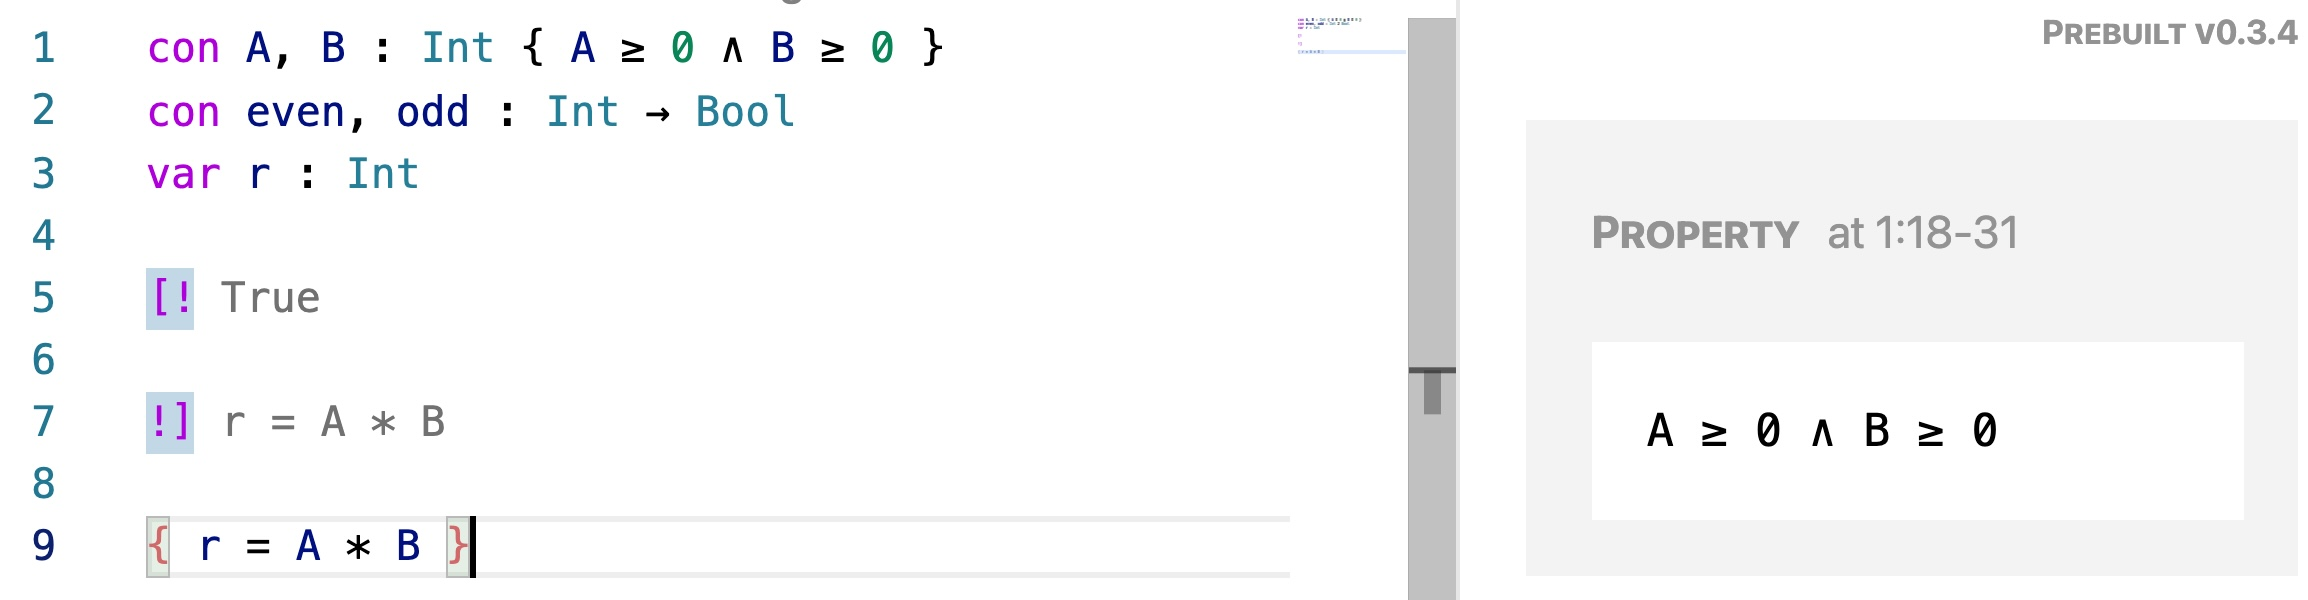
\includegraphics[width=\textwidth]{img/sshot00.jpg}
% \caption{Fast Multiplication in Guabao.}
% \label{fig:fastmul}
% \end{figure}

Guabao parses and analyses the code as it is typed into the editor.
Once the code is pasted into Guabao, we will see:\\
\sshotimg{sshot00}\\
Guabao automatically expands the question mark \ensuremath{\mathbin{?}} to a \emph{spec} — a hole in the program to be filled in, denoted by \ensuremath{[\mskip1.5mu \mathbin{!}\mathbin{...}\mathbin{!}\mskip1.5mu]}.
The idea of a spec is inspired by Morgan~\cite{Morgan:90:Programming}, with a slight difference: in Morgan~\cite{Morgan:90:Programming} one starts program construction from a spec with given pre/postconditions, while in Guabao the pre/postconditions are inferred.
The interface shows, on line 5 and 7, that code to be filled in shall bring the state of the system from precondition \ensuremath{\Conid{True}} to postcondition \ensuremath{\Varid{r}\mathrel{=}\Conid{A}\times\Conid{B}}. Properties of global constants (namely \ensuremath{\Conid{B}\geq \mathrm{0}}) are universally true and implicitly conjuncted with all assertions. They are displayed separately in a ``Property'' section in the right pane.

\paragraph{Introducing a Loop}
For such a non-trival task we expects that a loop is needed,
so we try to fill in the spec:
\\\sshotimg{sshot01}\\
Guabao syntactically enforces that each loop comes with a loop invariant and a bound.
Various techniques were developed to construct candidates of loop invariants from the postcondition.
We cannot properly cover the techniques in this paper but, for interested readers, we recommend Kaldewaij~\cite{Kaldewaij:90:Programming}.
For this problem, we use one of the standard tricks:
choose \ensuremath{\Varid{a}\times\Varid{b}\mathbin{+}\Varid{r}\mathrel{=}\Conid{A}\times\Conid{B}} as the loop invariant (line 7), which can be established by initialisation \ensuremath{\Varid{a},\Varid{b},\Varid{r}\mathbin{:=}\Conid{A},\Conid{B},\mathrm{0}} (line 6).
By letting the guard be \ensuremath{\Varid{b}\mathrel{\ne}\mathrm{0}} (line 8), the proof obligation {\sf InvBase} instantiates to \ensuremath{\Varid{a}\times\Varid{b}\mathbin{+}\Varid{r}\mathrel{=}\Conid{A}\times\Conid{B}\mathrel{\wedge}\Varid{b}\mathrel{=}\mathrm{0}\mathrel{\Rightarrow}\Varid{r}\mathrel{=}\Conid{A}\times\Conid{B}}, which is trivial to prove.
Now that the loop terminates when \ensuremath{\Varid{b}\mathrel{=}\mathrm{0}}, a strategy would be to keep decreasing \ensuremath{\Varid{b}} in the loop body until it reaches \ensuremath{\mathrm{0}},
therefore we let \ensuremath{\Varid{b}} be the bound (line 7).
The loop body is left as a question mark.

When the cursor is in the spec, press {\tt ctrl-c-r} to fill in the spec.
In the screenshot in Figure~\ref{fig:sshot2}, the code typed into the hole becomes part of the program,
while the question mark becomes a new hole.
\footnote{This style of interaction (including the hot-key combination) is inspired by Agda.}
The two POs shown on the right pane are respectively calculated {\sf InvBase} and {\sf TermBase}, while the pre/postconditions of the spec are calculated from {\sf InvInd}.
%\\\sshotimg{sshot02}\\

\begin{figure}[t]
\sshotimg{sshot02}\\
%\sshotimg{sshot03}
\caption{After introducing a loop.}
\label{fig:sshot2}
\end{figure}

\paragraph{The Interface}
Let us get a closer look at the interface of Guabao.
%Now it is a good time to inspect the interface of Guabao.
In the program in the left pane,
blue shade in the code indicates ``there are proof obligations incurred here.''
Program locations associated with more POs get a thicker shade.
The right pane contains information including
\begin{itemize}
\item inferred POs,
\item pre/postconditions of specs,
\item global properties, etc.
\end{itemize}
Since the number of POs can be large, in the right pane we display those on the path of the current location of the cursor.
In Figure~\ref{fig:sshot2}, the cursor is at line 7, beginning of the loop.
POs in the right pane include:
\begin{hscode}\linenumsetup\printlinebegin\SaveRestoreHook
\column{B}{@{}>{\hspre}l<{\hspost}@{}}%
\column{20}{@{}>{\hspre}l<{\hspost}@{}}%
\column{28}{@{}>{\hspre}l<{\hspost}@{}}%
\column{39}{@{}>{\hspre}c<{\hspost}@{}}%
\column{39E}{@{}l@{}}%
\column{44}{@{}>{\hspre}l<{\hspost}@{}}%
\column{55}{@{}>{\hspre}l<{\hspost}@{}}%
\column{E}{@{}>{\hspre}l<{\hspost}@{}}%
\>[B]{}\Varid{a}\times\Varid{b}\mathbin{+}\Varid{r}\mathrel{=}\Conid{A}\times\Conid{B}{}\<[20]%
\>[20]{}\mathrel{\wedge}\neg \;{}\<[28]%
\>[28]{}(\Varid{b}\mathrel{\ne}\mathrm{0}){}\<[39]%
\>[39]{}\mathrel{\Rightarrow}{}\<[39E]%
\>[44]{}\Varid{r}\mathrel{=}\Conid{A}\times\Conid{B}{}\<[55]%
\>[55]{}~~, \mbox{which is {\sf InvBase}, and}{}\<[E]%
\printlineend\\
\printlinebegin\>[B]{}\Varid{a}\times\Varid{b}\mathbin{+}\Varid{r}\mathrel{=}\Conid{A}\times\Conid{B}{}\<[20]%
\>[20]{}\mathrel{\wedge}{}\<[28]%
\>[28]{}\Varid{b}\mathrel{\ne}\mathrm{0}{}\<[39]%
\>[39]{}\mathrel{\Rightarrow}{}\<[39E]%
\>[44]{}\Varid{b}\geq \mathrm{0}{}\<[55]%
\>[55]{}~~, \mbox{which is {\sf TermBase}}.{}\<[E]%
\printlineend\ColumnHook
\end{hscode}\resethooks
%The first one is aforementioned {\sf InvBase}, while the second is {\sf TermBase}.

The {\sf InvBase} PO is trivial to prove --- the invariant and the bound were designed to make it trivial.
At the top of the box displaying this PO there is a icons of a magic wand.
Clicking on it invokes the SMT solver Z3, which generates the output "Q.E.D", indicated that it is proved.
The PO {\sf TermBase}, however, turns out to be falsifiable. Indeed, the premise does not guarantee \ensuremath{\Varid{b}\geq \mathrm{0}}! We thus realise that we need a stronger invariant. The new invariant would be:
\begin{hscode}\linenumsetup\printlinebegin\SaveRestoreHook
\column{B}{@{}>{\hspre}l<{\hspost}@{}}%
\column{21}{@{}>{\hspre}c<{\hspost}@{}}%
\column{21E}{@{}l@{}}%
\column{25}{@{}>{\hspre}l<{\hspost}@{}}%
\column{E}{@{}>{\hspre}l<{\hspost}@{}}%
\>[B]{}\Varid{a}\times\Varid{b}\mathbin{+}\Varid{r}\mathrel{=}\Conid{A}\times\Conid{B}{}\<[21]%
\>[21]{}\mathrel{\wedge}{}\<[21E]%
\>[25]{}\Varid{b}\geq \mathrm{0}~~.{}\<[E]%
\printlineend\ColumnHook
\end{hscode}\resethooks
After the user updates the invariant, the POs and the specs are updated accordingly.

% Each PO comes with a hash key. Clicking on the hash key for the first PO, for example, results in the screenshot in the bottom of Figure~\ref{fig:sshot23}.
% %\\\sshotimg{sshot03}\\
% A new comment block having the hash key is added to the bottom of the code, in which the programmer can write up a proof of the corresponding property.
% A program is proven correct if all POs are proved.
% Hash key of a PO with a proof block is displayed in blue (see the top-right corner).
% Currently the system makes no attempt to check these proofs, however.
% They are just comments for the user.


\paragraph{Constructing the Loop Body}
Now we attempt to construct the loop body.
Having {\sf TermInd} in mind, one of the objective of the loop is to decrease the bound \ensuremath{\Varid{b}} and thereby construct a loop that terminates.
There are various ways to do so.
One may decrement \ensuremath{\Varid{b}} by \ensuremath{\Varid{b}\mathbin{:=}\Varid{b}\mathbin{-}\mathrm{1}}, or one may divide \ensuremath{\Varid{b}} by half --- knowing that \ensuremath{\Varid{b}} is not zero.
Let us try the second way. We type
\begin{hscode}\linenumsetup\printlinebegin\SaveRestoreHook
\column{B}{@{}>{\hspre}l<{\hspost}@{}}%
\column{E}{@{}>{\hspre}l<{\hspost}@{}}%
\>[B]{}\mathbin{?}{}\<[E]%
\printlineend\\
\printlinebegin\>[B]{}\Varid{b}\mathbin{:=}\Varid{b}\mathbin{/}\mathrm{2}{}\<[E]%
\printlineend\ColumnHook
\end{hscode}\resethooks
into the spec.
In effect, we are trying to construct a block of statements by guessing that the \emph{last} statement could be \ensuremath{\Varid{b}\mathbin{:=}\Varid{b}\mathbin{/}\mathrm{2}}, and think about what should come before it.
Note that the operator \ensuremath{\mathbin{/}} here denotes integral division, which rounds down to the closest integer.
Pressing {\tt ctrl-c-r}, the question mark gets expanded to a spec with an updated postcondition (top of Figure~\ref{fig:sshot45}).
The spec expects us to fill in some code that brings the computer from a state satisfying
\begin{hscode}\linenumsetup\printlinebegin\SaveRestoreHook
\column{B}{@{}>{\hspre}l<{\hspost}@{}}%
\column{E}{@{}>{\hspre}l<{\hspost}@{}}%
\>[B]{}\Varid{a}\times\Varid{b}\mathbin{+}\Varid{r}\mathrel{=}\Conid{A}\times\Conid{B}\mathrel{\wedge}\Varid{b}\geq \mathrm{0}\mathrel{\wedge}\Varid{b}\mathrel{\ne}\mathrm{0}{}\<[E]%
\printlineend\ColumnHook
\end{hscode}\resethooks
to a state satisfying
\begin{hscode}\linenumsetup\printlinebegin\SaveRestoreHook
\column{B}{@{}>{\hspre}l<{\hspost}@{}}%
\column{E}{@{}>{\hspre}l<{\hspost}@{}}%
\>[B]{}\Varid{a}\times(\Varid{b}\mathbin{/}\mathrm{2})\mathbin{+}\Varid{r}\mathrel{=}\Conid{A}\times\Conid{B}\mathrel{\wedge}\Varid{b}\mathbin{/}\mathrm{2}\geq \mathrm{0}~~.{}\<[E]%
\printlineend\ColumnHook
\end{hscode}\resethooks
What can we do?

\begin{figure}[th]
\sshotimg{sshot04}\\
\sshotimg{sshot05}
\caption{Top: guessing that the last statement could be \ensuremath{\Varid{b}\mathbin{:=}\Varid{b}\mathbin{/}\mathrm{2}}.
Bottom: trying to fill in \ensuremath{\Varid{b}\mathbin{:=}\Varid{b}\times\mathrm{2}} in the loop body --- we cannot prove the PO.}
\label{fig:sshot45}
\end{figure}

One possibility is filling in \ensuremath{\Varid{b}\mathbin{:=}\Varid{b}\times\mathrm{2}}.
That, however, results in the bottom of Figure~\ref{fig:sshot45}, where the PO shown in the right pane, which is a consequence of {\sf TermInd} demands us to prove that
\begin{hscode}\linenumsetup\printlinebegin\SaveRestoreHook
\column{B}{@{}>{\hspre}l<{\hspost}@{}}%
\column{E}{@{}>{\hspre}l<{\hspost}@{}}%
\>[B]{}\mathbin{....}\Varid{b}\mathrel{=}{?bnd_{51}}\mathbin{...}\mathrel{\Rightarrow}(\Varid{b}\times\mathrm{2})\mathbin{/}\mathrm{2}\mathbin{<}{?bnd_{51}}~~,{}\<[E]%
\printlineend\ColumnHook
\end{hscode}\resethooks
where \ensuremath{{?bnd_{51}}} is a system-generated logical variable.
This property cannot be proved, and
we learn that \ensuremath{\Varid{b}\mathbin{:=}\Varid{b}\times\mathrm{2};\Varid{b}\mathbin{:=}\Varid{b}\mathbin{/}\mathrm{2}} is a bad idea as the loop body --- the bound \ensuremath{\Varid{b}} does not decrease.

Another possible choice is \ensuremath{\Varid{a}\mathbin{:=}\Varid{a}\times\mathrm{2}}. If we try this option:\\
\sshotimg{sshot06}\\
It turns out that we have to prove a PO that simplifies to
\begin{hscode}\linenumsetup\printlinebegin\SaveRestoreHook
\column{B}{@{}>{\hspre}l<{\hspost}@{}}%
\column{36}{@{}>{\hspre}l<{\hspost}@{}}%
\column{E}{@{}>{\hspre}l<{\hspost}@{}}%
\>[B]{}(\Varid{a}\times\Varid{b})\mathbin{+}\Varid{r}\mathrel{=}\Conid{A}\times\Conid{B}\mathbin{....}~~{}\<[36]%
\>[36]{}\mathrel{\Rightarrow}~~((\Varid{a}\times\mathrm{2})\times(\Varid{b}\mathbin{/}\mathrm{2}))\mathbin{+}\Varid{r}\mathrel{=}\Conid{A}\times\Conid{B}\mathbin{....}{}\<[E]%
\printlineend\ColumnHook
\end{hscode}\resethooks
This time we demonstrate a manual proof.
Each PO comes with a hash key.
Clicking on the hash key ({\sf \#5F2E722} in the screenshot above) for the PO creates
a new comment block labelled by the hash key, in which the programmer can write
up a proof of the corresponding property.
Hash key of a PO with a proof block is displayed in blue.
A program is proven correct if all POs are either proved by Z3 or by the programmer.

Currently the system makes no attempt to check the proofs written by the user ---
in a lecture the proofs would be checked by a teacher.
It is our future work to develop a language that is suitable for manual calculational proofs and yet machine-verifiable.

% They are just comments for the user.
% Hash key of a PO with a proof block is displayed in blue (see the top-right corner).
%

It turns out that, to prove the PO, we will need \ensuremath{\Varid{b}} to be a even number (line 17 in the screenshot), assuming integral division.
This is a hint that we shall wrap \ensuremath{\Varid{a}\mathbin{:=}\Varid{a}\times\mathrm{2};\Varid{b}\mathbin{:=}\Varid{b}\mathbin{/}\mathrm{2}} in a guard \ensuremath{\Varid{even}\;\Varid{b}}, to ensure that \ensuremath{\Varid{b}} is even, and put it in an \ensuremath{\mathbf{if}} construct.
The current code is:
\begin{hscode}\linenumsetup\printlinebegin\SaveRestoreHook
\column{B}{@{}>{\hspre}l<{\hspost}@{}}%
\column{3}{@{}>{\hspre}l<{\hspost}@{}}%
\column{17}{@{}>{\hspre}l<{\hspost}@{}}%
\column{E}{@{}>{\hspre}l<{\hspost}@{}}%
\>[B]{}\mathbf{do}\;\Varid{b}\mathrel{\ne}\mathrm{0}\to {}\<[E]%
\printlineend\\
\printlinebegin\>[B]{}\hsindent{3}{}\<[3]%
\>[3]{}\mathbf{if}\;\Varid{even}\;\Varid{b}\to {}\<[17]%
\>[17]{}\Varid{a}\mathbin{:=}\Varid{a}\times\mathrm{2}{}\<[E]%
\printlineend\\
\printlinebegin\>[17]{}\Varid{b}\mathbin{:=}\Varid{b}\mathbin{/}\mathrm{2}{}\<[E]%
\printlineend\\
\printlinebegin\>[B]{}\hsindent{3}{}\<[3]%
\>[3]{}\mathbf{fi}{}\<[E]%
\printlineend\\
\printlinebegin\>[B]{}\mathbf{od}~~.{}\<[E]%
\printlineend\ColumnHook
\end{hscode}\resethooks

\paragraph{Totalisation}
We are not done yet. Among all the POs we will be asked to prove that \ensuremath{\mathbf{if}} is total --- every possible case is covered.
Therefore we need to think about what to do in the \ensuremath{\Varid{odd}\;\Varid{b}} case. For this case we might decrease \ensuremath{\Varid{b}} by \ensuremath{\Varid{b}\mathbin{:=}\Varid{b}\mathbin{-}\mathrm{1}}. By a similar process we can construct what to do with \ensuremath{\Varid{a}} and \ensuremath{\Varid{r}} in this case to maintain the invariant. A possible final program would be (omitting the declarations):
\begin{hscode}\linenumsetup\printlinebegin\SaveRestoreHook
\column{B}{@{}>{\hspre}l<{\hspost}@{}}%
\column{15}{@{}>{\hspre}l<{\hspost}@{}}%
\column{19}{@{}>{\hspre}l<{\hspost}@{}}%
\column{27}{@{}>{\hspre}c<{\hspost}@{}}%
\column{27E}{@{}l@{}}%
\column{31}{@{}>{\hspre}l<{\hspost}@{}}%
\column{E}{@{}>{\hspre}l<{\hspost}@{}}%
\>[B]{}\Varid{a},\Varid{b},\Varid{r}\mathbin{:=}\Conid{A},\Conid{B},\mathrm{0}{}\<[E]%
\printlineend\\
\printlinebegin\>[B]{}\assert{\Varid{a}\times\Varid{b}\mathbin{+}\Varid{r}\mathrel{=}\Conid{A}\times\Conid{B}\mathrel{\wedge}\Varid{b}\geq \mathrm{0},\Varid{bnd}\mathbin{:}\Varid{b}}{}\<[E]%
\printlineend\\
\printlinebegin\>[B]{}\mathbf{do}\;\Varid{b}\mathrel{\ne}\mathrm{0}\to {}\<[15]%
\>[15]{}\mathbf{if}\;{}\<[19]%
\>[19]{}\Varid{even}\;\Varid{b}{}\<[27]%
\>[27]{}\to {}\<[27E]%
\>[31]{}\Varid{a}\mathbin{:=}\Varid{a}\times\mathrm{2}{}\<[E]%
\printlineend\\
\printlinebegin\>[31]{}\Varid{b}\mathbin{:=}\Varid{b}\mathbin{/}\mathrm{2}{}\<[E]%
\printlineend\\
\printlinebegin\>[15]{}\mid {}\<[19]%
\>[19]{}\Varid{odd}\;\Varid{b}{}\<[27]%
\>[27]{}\to {}\<[27E]%
\>[31]{}\Varid{r}\mathbin{:=}\Varid{a}\mathbin{+}\Varid{r}{}\<[E]%
\printlineend\\
\printlinebegin\>[31]{}\Varid{b}\mathbin{:=}\Varid{b}\mathbin{-}\mathrm{1}{}\<[E]%
\printlineend\\
\printlinebegin\>[15]{}\mathbf{fi}{}\<[E]%
\printlineend\\
\printlinebegin\>[B]{}\mathbf{od}{}\<[E]%
\printlineend\\
\printlinebegin\>[B]{}\assert{\Varid{r}\mathrel{=}\Conid{A}\times\Conid{B}}~~,{}\<[E]%
\printlineend\ColumnHook
\end{hscode}\resethooks
which computes \ensuremath{\Conid{A}\times\Conid{B}} using $O(\log B)$ atomic arithmetic operations.

But that is not the only possible program. One might decide to do nothing in the \ensuremath{\Varid{odd}\;\Varid{b}} case and always decrease \ensuremath{\Varid{b}} regardless of its parity, resulting in:

\begin{hscode}\linenumsetup\printlinebegin\SaveRestoreHook
\column{B}{@{}>{\hspre}l<{\hspost}@{}}%
\column{15}{@{}>{\hspre}l<{\hspost}@{}}%
\column{19}{@{}>{\hspre}l<{\hspost}@{}}%
\column{30}{@{}>{\hspre}l<{\hspost}@{}}%
\column{E}{@{}>{\hspre}l<{\hspost}@{}}%
\>[B]{}\Varid{a},\Varid{b},\Varid{r}\mathbin{:=}\Conid{A},\Conid{B},\mathrm{0}{}\<[E]%
\printlineend\\
\printlinebegin\>[B]{}\assert{\Varid{a}\times\Varid{b}\mathbin{+}\Varid{r}\mathrel{=}\Conid{A}\times\Conid{B}\mathrel{\wedge}\Varid{b}\geq \mathrm{0},\Varid{bnd}\mathbin{:}\Varid{b}}{}\<[E]%
\printlineend\\
\printlinebegin\>[B]{}\mathbf{do}\;\Varid{b}\mathrel{\ne}\mathrm{0}\to {}\<[15]%
\>[15]{}\Varid{r}\mathbin{:=}\Varid{a}\mathbin{+}\Varid{r}{}\<[E]%
\printlineend\\
\printlinebegin\>[15]{}\Varid{b}\mathbin{:=}\Varid{b}\mathbin{-}\mathrm{1}{}\<[E]%
\printlineend\\
\printlinebegin\>[15]{}\mathbf{if}\;{}\<[19]%
\>[19]{}\Varid{even}\;\Varid{b}\to {}\<[30]%
\>[30]{}\Varid{a}\mathbin{:=}\Varid{a}\times\mathrm{2}{}\<[E]%
\printlineend\\
\printlinebegin\>[30]{}\Varid{b}\mathbin{:=}\Varid{b}\mathbin{/}\mathrm{2}{}\<[E]%
\printlineend\\
\printlinebegin\>[15]{}\mid {}\<[19]%
\>[19]{}\Varid{odd}\;\Varid{b}\to {}\<[30]%
\>[30]{}\Varid{skip}{}\<[E]%
\printlineend\\
\printlinebegin\>[15]{}\mathbf{fi}{}\<[E]%
\printlineend\\
\printlinebegin\>[B]{}\mathbf{od}{}\<[E]%
\printlineend\\
\printlinebegin\>[B]{}\assert{\Varid{r}\mathrel{=}\Conid{A}\times\Conid{B}}~~.{}\<[E]%
\printlineend\ColumnHook
\end{hscode}\resethooks
The program is correct as long as one can prove all the POs.

\paragraph{Summary}
Let us recapitulate the interaction between a program and its proof in this example.
Certainly, the program determines what ought to be proved --- introducing a statement also introduces corresponding POs.
Meanwhile, these POs also gave hints on how to proceed with program construction.
One may design the program --- for example, choosing the loop guard or choosing a method to decrease the bound --- such that some POs are trivial to discharge.
Pre/postconditions of a spec, inferred from future POs, shows what a piece of code is supposed to do.
By observing what is missing in an attempted proof, one may learn how to strengthen the loop invariant, to enclose the program fragment in a guard, or learn that the current choice is simply wrong.
The interface of Guabao aims to encourage such interaction.

% \begin{figure}
%   \centering
%      \begin{subfigure}[b]{0.3\textwidth}
%        here
%        \caption{$y=x$}
%      \end{subfigure}
%      \begin{subfigure}[b]{0.3\textwidth}
%        there
%        \caption{$y=x$}
%      \end{subfigure}
% \end{figure}


\begin{figure}[th]
\sshotimg{mss}
\caption{The \emph{maximum segment sum} problem.}
\label{fig:mss}
\end{figure}

\paragraph{Other Features}
Figure~\ref{fig:mss} presents the classical \emph{maximum segment sum} problem, which demonstrates some features we have not mentioned in the previous example.
Given an array of \ensuremath{\Conid{N}} integers (line 2), the goal is to find the maximum possible some of a consecutive segment.
The postcondition on line 17 formally describes the goal --- see the use of Eindhoven notation for quantifiers, which denotes ``for \ensuremath{\mathrm{0}\leq \Varid{i}\leq \Varid{j}\leq \Conid{N}}, collect \ensuremath{\Varid{sum}\;\Varid{i}\;\Varid{j}} and find the largest \ensuremath{(\mathbin{\uparrow})},  where \ensuremath{\Varid{i}} and \ensuremath{\Varid{j}} are bound variables.''
Guabao supports arrays that can be nested and mutable (if declared in \ensuremath{\mathbf{var}}).
Pure functions to be used in assertions can be defined in declaration blocks \ensuremath{\{\mskip1.5mu \mathbin{:}\mathbin{...}\mathbin{:}\mskip1.5mu\}}.
Shown in the right pane a PO induced from {\sf InvInd} --- that the invariant holds after one more iteration of the loop.
The notation \ensuremath{\Conid{P}\;\lbrack\Varid{s}\backslash\Varid{s}\mathbin{\uparrow}\Varid{r}\rbrack} denotes substituting \ensuremath{\Varid{s}\mathbin{\uparrow}\Varid{r}} for all free occurrences of \ensuremath{\Varid{s}} in \ensuremath{\Conid{P}}, which appears in the PO as a consequences of \ensuremath{\Varid{s}\mathbin{:=}\Varid{s}\mathbin{\uparrow}\Varid{r}} in the code. Clicking on \ensuremath{\Conid{P}} expands its definition and performs the substitution.

Like the previous example, development of this program was not done in one step.
The usual story goes like: we started with a spec without \ensuremath{\Varid{r}}, using \ensuremath{\Conid{P}\mathrel{\wedge}\mathrm{0}\leq \Varid{n}\leq \Conid{N}} as the loop invariant, and the first attempt was to construct the main loop with \ensuremath{\Varid{n}\mathbin{:=}\Varid{n}\mathbin{+}\mathrm{1}} as its \emph{last} step. While trying to satisfy the spec and prove {\sf InvInd}, we would discover that, to update \ensuremath{\Varid{s}} quickly, we may strengthen the invariant with a variable \ensuremath{\Varid{r}}, storing the maximum \emph{suffix} sum, as stated by \ensuremath{\Conid{Q}\;\Varid{n}}, which was also discovered during the proof. The interface of Guabao wishes to make this process natural and smooth.

\section{Behind the Scenes}
\label{sec:po-generation}

A central part of the backend of Guabao is an engine that scans through the code, generates a collection of POs, and infers the pre/post conditions of specs.
In this section we examine the design of this engine.

When seeing a Hoare triple \ensuremath{\htriple{\Conid{P}}{\Conid{S}}{\Conid{Q}}}, Guabao invokes the ternary function \ensuremath{\lBrace\anonymous \rBrace\,\anonymous \,\lBrace\anonymous \rBrace}, summarised in Figure~\ref{fig:struct}, to generate POs.
The function \ensuremath{\lBrace\anonymous \rBrace\,\anonymous \,\lBrace\anonymous \rBrace} will be discussed in more details later.
To understand it, however, we shall start with some discussion on the interplay between assertions and POs.
%\todo{Briefly describe the relation of wp, assertions and PO}
%something like: "The algorithm generating POs is described below: it involves the concept of weakest precondition and how the programmer places the assertions among the program"
%SCM: but that's what I am going to discuss. I added a sentence: The function |struct _ _ _| will be discussed in more details later.


\paragraph{Weakest preconditions}
It is known that for every statement \ensuremath{\Conid{S}}, one can compute \ensuremath{\Varid{wp}\;\Conid{S}\;\Conid{Q}}, its weakest precondition with respect to postcondition \ensuremath{\Conid{Q}}.
Our definition of \ensuremath{\Varid{wp}} is shown in Figure~\ref{fig:wp}.
The first few cases are standard: \ensuremath{\Varid{wp}\;\Varid{abort}\;\Conid{Q}} is always \ensuremath{\Conid{False}}, \ensuremath{\Varid{wp}\;\Varid{skip}} is the identity function, and \ensuremath{\Varid{wp}\;(\Varid{x}\mathbin{:=}\Varid{e})} is substitution --- \ensuremath{\Conid{Q}\;\lbrack\Varid{x}\backslash\Varid{e}\rbrack} denotes substituting all free occurrences of \ensuremath{\Varid{x}} in \ensuremath{\Conid{Q}} by \ensuremath{\Varid{e}}.
The cases for \ensuremath{\mathbf{if}} and \ensuremath{\mathbf{do}} statements are also standard --- for clarity we present instances containing two guarded commands.

A sequence of statements \ensuremath{\Conid{S}_{0};\mathinner{\ldotp\ldotp};\Conid{Sn}} operationally denotes performing the statements in the given order.
We extend the notion to allow assertions and specs in the sequence.
In the patterns between line \ref{code:wp:seq:0} -- \ref{code:wp:seq:3} in Figure~\ref{fig:wp},
\ensuremath{(\{\mskip1.5mu \Conid{P}\mskip1.5mu\}\;\Conid{Ss})} denotes a sequence starting with an assertion,
\ensuremath{(\lbrack!~!\rbrack\;\Conid{Ss})} denotes one starting with a spec,
and \ensuremath{(\Varid{s};\Varid{ss})} a sequence starting with a non-sequent statement followed by sequence \ensuremath{\Varid{ss}}.
An empty sequence is denoted by \ensuremath{\epsilon}, and \ensuremath{\Varid{wp}\;\epsilon} is the identity function.
For the \ensuremath{(\Varid{s};\Varid{ss})} case, we have the standard definition \ensuremath{\Varid{wp}\;(\Varid{s};\Varid{ss})\;\Conid{Q}\mathrel{=}\Varid{wp}\;\Varid{s}\;(\Varid{wp}\;\Varid{ss}\;\Conid{Q})}.
%\todo{Reorganize the paragraph}
%something like: “The cases above are rules upon a single statement; since a program is usually constituted with a sequence of statements, we use the rules 7-10, to denote assertions and specs regarding a statement sequence. |({P} Ss)| denotes...”
%SCM: I tried to refrain from categorising the previous cases as "single statements" since IF and DO are both compound statements.

The last two cases on line \ref{code:wp:seq:2} -- \ref{code:wp:seq:3} reveal that \ensuremath{\Varid{wp}} actually returns a monadic value.
For brevity we have pretended that \ensuremath{\Varid{wp}} returns a pure value in previous cases,
omitted the Haskell-ish \ensuremath{\mathbf{do}} keyword,
and spelled out the keyword \ensuremath{\Varid{return}} only when it follows an effectful operation.
More about these two cases will be discussed later.
%\todo{Reorganize the paragraph}
%something like: “|wp| is actually returning a monadic value. For brevity, we have pretended that |wp| returns a pure value in simpler cases(line1-8); when it involves effectful operations -- tellPO and tellSpec, which can be seen in the last two rules --, we explicitly spell out the keyword |return|, omitting the Haskell-ish |do| keyword.”
%SCM: We used return in line 10 too, which does not contain tellPO and tellSpec.

% this is how I see the logical flow of these 3 paragraphs: from dealing with simple cases to its true, monadic nature.

\begin{figure}[t]
\numberson
\begin{hscode}\linenumsetup\printlinebegin\SaveRestoreHook
\column{B}{@{}>{\hspre}l<{\hspost}@{}}%
\column{3}{@{}>{\hspre}l<{\hspost}@{}}%
\column{13}{@{}>{\hspre}l<{\hspost}@{}}%
\column{14}{@{}>{\hspre}l<{\hspost}@{}}%
\column{16}{@{}>{\hspre}l<{\hspost}@{}}%
\column{18}{@{}>{\hspre}l<{\hspost}@{}}%
\column{21}{@{}>{\hspre}l<{\hspost}@{}}%
\column{34}{@{}>{\hspre}l<{\hspost}@{}}%
\column{36}{@{}>{\hspre}c<{\hspost}@{}}%
\column{36E}{@{}l@{}}%
\column{49}{@{}>{\hspre}l<{\hspost}@{}}%
\column{E}{@{}>{\hspre}l<{\hspost}@{}}%
\>[B]{}\Varid{wp}\;\Varid{abort}\;{}\<[14]%
\>[14]{}\Conid{Q}\mathrel{=}\Conid{False}{}\<[E]%
\printlineend\\
\printlinebegin\>[B]{}\Varid{wp}\;\Varid{skip}\;{}\<[14]%
\>[14]{}\Conid{Q}\mathrel{=}\Varid{skip}{}\<[E]%
\printlineend\\
\printlinebegin\>[B]{}\Varid{wp}\;(\Varid{x}\mathbin{:=}\Varid{e})\;{}\<[14]%
\>[14]{}\Conid{Q}\mathrel{=}\Conid{Q}\;\lbrack\Varid{x}\backslash\Varid{e}\rbrack{}\<[E]%
\printlineend\\
\printlinebegin\>[B]{}\Varid{wp}\;(\mathbf{if}\;\Conid{B}_{0}\to \Conid{S}_{0}{}\<[18]%
\>[18]{}\mid \Conid{B}_{1}\to \Conid{S}_{1}\;\mathbf{fi})\;\Conid{Q}{}\<[36]%
\>[36]{}\mathrel{=}{}\<[36E]%
\printlineend\\
\printlinebegin\>[B]{}\hsindent{3}{}\<[3]%
\>[3]{}(\Conid{B}_{0}\mathrel{\vee}\Conid{B}_{1})\mathrel{\wedge}(\Conid{B}_{0}\Rightarrow \Varid{wp}\;\Conid{S}_{0}\;\Conid{Q})\mathrel{\wedge}(\Conid{B}_{1}\Rightarrow \Varid{wp}\;\Conid{S}_{1}\;\Conid{Q}){}\<[E]%
\printlineend\\
\printlinebegin\>[B]{}\Varid{wp}\;(\mathbf{do}\;\Conid{B}_{0}\to \Conid{S}_{0}{}\<[18]%
\>[18]{}\mid \Conid{B}_{1}\to \Conid{S}_{1}\;\mathbf{od})\;{}\<[34]%
\>[34]{}\Conid{Q}\mathrel{=}{}\<[E]%
\printlineend\\
\printlinebegin\>[B]{}\hsindent{3}{}\<[3]%
\>[3]{}\mu\;(\Conid{X}\to ((\Conid{B}_{0}\mathrel{\wedge}\Conid{B}_{1})\mathrel{\vee}\Conid{Q})\mathrel{\wedge}(\Conid{B}_{0}\Rightarrow \Varid{wp}\;\Conid{S}_{0}\;\Conid{X})\mathrel{\wedge}(\Conid{B}_{1}\Rightarrow \Varid{wp}\;\Conid{S}_{1}\;\Conid{X})){}\<[E]%
\printlineend\\[\blanklineskip]%
\printlinebegin\>[B]{}\Varid{wp}\;\epsilon\;{}\<[13]%
\>[13]{}\Conid{Q}\mathrel{=}\Conid{Q}{}\<[49]%
\>[49]{}\label{code:wp:seq:0}{}\<[E]%
\printlineend\\
\printlinebegin\>[B]{}\Varid{wp}\;(\Varid{s};\Varid{ss})\;{}\<[13]%
\>[13]{}\Conid{Q}\mathrel{=}\Varid{wp}\;\Varid{s}\;(\Varid{wp}\;\Varid{ss}\;\Conid{Q}){}\<[E]%
\printlineend\\[\blanklineskip]%
\printlinebegin\>[B]{}\Varid{wp}\;(\{\mskip1.5mu \Conid{P}\mskip1.5mu\}\;\Conid{Ss})\;{}\<[16]%
\>[16]{}\Conid{Q}\mathrel{=}\lBrace\Conid{P}\rBrace\,\Conid{Ss}\,\lBrace\Conid{Q}\rBrace;\Varid{return}\;\Conid{P}{}\<[49]%
\>[49]{}\label{code:wp:seq:2}{}\<[E]%
\printlineend\\
\printlinebegin\>[B]{}\Varid{wp}\;(\lbrack!~!\rbrack\;\Conid{Ss})\;{}\<[16]%
\>[16]{}\Conid{Q}\mathrel{=}{}\<[21]%
\>[21]{}\Conid{Q'}\leftarrow \Varid{wp}\;\Conid{Ss}\;\Conid{Q}{}\<[49]%
\>[49]{}\label{code:wp:seq:3}{}\<[E]%
\printlineend\\
\printlinebegin\>[21]{}\Varid{tellSpec}\;[\mskip1.5mu \mathbin{!}\Conid{Q'},\Conid{Q'}\mathbin{!}\mskip1.5mu]{}\<[E]%
\printlineend\\
\printlinebegin\>[21]{}\Varid{return}\;\Conid{Q'}{}\<[E]%
\printlineend\ColumnHook
\end{hscode}\resethooks
%wp (IF B0 -> S0  | B1 -> S1 FI) Q  = (B0 || B1) && (Bi => wp Si Q)
\numbersoff
\numbersreset
\caption{The weakest precondition predicate transformer.}
\label{fig:wp}
\end{figure}

\paragraph{Assertions and POs}
The conventional definition of a Hoare triple is \ensuremath{\htriple{\Conid{P}}{\Conid{S}}{\Conid{Q}}\,\mathrel{=}\,(\Conid{P}\mathrel{\Rightarrow}\Varid{wp}\;\Conid{S}\;\Conid{Q})}.
The main programs in Guabao also come in the form \ensuremath{\htriple{\Conid{P}}{\Conid{S}}{\Conid{Q}}}.
To establish the correctness of a completed program, we could simply let the PO be the monolithic property \ensuremath{\Conid{P}\mathrel{\Rightarrow}\Varid{wp}\;\Conid{S}\;\Conid{Q}}.
However, this is not helpful for program construction.
%because this would be the same as splitting program construction and proof of correctness.
%SCM: hmm.. the reason is more subtle.
We wish to produce POs that give hints to each program component that needs to be constructed.
PO generation is therefore an design issue:
we want to generate POs that are useful for program construction, and moderate in size and number.

On one thing, according to Figure~\ref{fig:wp}, a PO can be broken down along the structure of the program.
On another, given a sequence of statements, how assertions are placed reflects the intention of the programmer.
For example, given the program fragment below:
\begin{hscode}\linenumsetup\printlinebegin\SaveRestoreHook
\column{B}{@{}>{\hspre}l<{\hspost}@{}}%
\column{35}{@{}>{\hspre}l<{\hspost}@{}}%
\column{E}{@{}>{\hspre}l<{\hspost}@{}}%
\>[B]{}\htripletwo{\Conid{P}}{\Conid{S}_{0};\Conid{S}_{1}}{\Conid{R}}{\Conid{S}_{2};\Conid{S}_{3}}{\Conid{Q}}{}\<[35]%
\>[35]{}~~,{}\<[E]%
\printlineend\ColumnHook
\end{hscode}\resethooks
where \ensuremath{\Conid{S}_{0}} -- \ensuremath{\Conid{S}_{3}} are statements containing no assertions or specs.
%SCM: The previous line cannot be omitted. Otherwise Guabao would not generate the PO below as claimed.
This could be reflecting the intention that, at the point between \ensuremath{\Conid{S}_{1}} and \ensuremath{\Conid{S}_{2}},
the programmer wishes to conclude all the information about the current state, which can be used to prove the correctness of the former and the latter part of the program separately.
Therefore, Guabao should emit two POs: \ensuremath{\Conid{R}\mathrel{\Rightarrow}\Varid{wp}\;\Conid{S}_{2}\;(\Varid{wp}\;\Conid{S}_{3}\;\Conid{Q})}, and \ensuremath{\Conid{P}\mathrel{\Rightarrow}\Varid{wp}\;\Conid{S}_{0}\;(\Varid{wp}\;\Conid{S}_{1}\;\Conid{R})}.

Note that this is stronger than the traditional definition:
\ensuremath{\Varid{wp}\;\assert{\Conid{R}}\;\Conid{Q}\mathrel{=}\Conid{R}\mathrel{\wedge}\Conid{Q}}.
Consider the following programs (assuming \ensuremath{\Varid{x},\Varid{z}\mathbin{:}\Conid{Int}}):
\begin{hscode}\linenumsetup\printlinebegin\SaveRestoreHook
\column{B}{@{}>{\hspre}l<{\hspost}@{}}%
\column{25}{@{}>{\hspre}l<{\hspost}@{}}%
\column{E}{@{}>{\hspre}l<{\hspost}@{}}%
\>[B]{}{\sf P}_0:\qquad{}\<[25]%
\>[25]{}\{\mskip1.5mu \Varid{z}\mathbin{>}\Varid{x}\mskip1.5mu\}\;\Varid{x}\mathbin{:=}\Varid{z}\mathbin{-}\Varid{x};\Varid{x}\mathbin{:=}\Varid{x}\mathbin{/}\mathrm{2}\;\{\mskip1.5mu \Varid{x}\geq \mathrm{0}\mskip1.5mu\}~~,{}\<[E]%
\printlineend\\
\printlinebegin\>[B]{}{\sf P}_1:\qquad{}\<[25]%
\>[25]{}\{\mskip1.5mu \Varid{z}\mathbin{>}\Varid{x}\mskip1.5mu\}\;\Varid{x}\mathbin{:=}\Varid{z}\mathbin{-}\Varid{x}\;\{\mskip1.5mu \Varid{x}\mathbin{>}\mathrm{0}\mskip1.5mu\}\;\Varid{x}\mathbin{:=}\Varid{x}\mathbin{/}\mathrm{2}\;\{\mskip1.5mu \Varid{x}\geq \mathrm{0}\mskip1.5mu\}~~,{}\<[E]%
\printlineend\\
\printlinebegin\>[B]{}{\sf P}_2:\qquad{}\<[25]%
\>[25]{}\{\mskip1.5mu \Varid{z}\mathbin{>}\Varid{x}\mskip1.5mu\}\;\Varid{x}\mathbin{:=}\Varid{z}\mathbin{-}\Varid{x}\;\{\mskip1.5mu \Conid{True}\mskip1.5mu\}\;\Varid{x}\mathbin{:=}\Varid{x}\mathbin{/}\mathrm{2}\;\{\mskip1.5mu \Varid{x}\geq \mathrm{0}\mskip1.5mu\}~~.{}\<[E]%
\printlineend\ColumnHook
\end{hscode}\resethooks
Program ${\sf P}_0$ generates one PO: \ensuremath{\Varid{z}\mathbin{>}\Varid{x}\mathrel{\Rightarrow}(\Varid{z}\mathbin{-}\Varid{x})\mathbin{/}\mathrm{2}\geq \mathrm{0}}, while ${\sf P}_1$ generates two POs: \ensuremath{\Varid{x}\mathbin{>}\mathrm{0}\mathrel{\Rightarrow}\Varid{x}\mathbin{/}\mathrm{2}\geq \mathrm{0}} and \ensuremath{\Varid{z}\mathbin{>}\Varid{x}\mathrel{\Rightarrow}\Varid{z}\mathbin{-}\Varid{x}\mathbin{>}\mathrm{0}}.
All of them can easily be discharged.
In contrast, while ${\sf P}_2$ is a valid program in the traditional setting, Guabao would generate an unprovable PO: \ensuremath{\Conid{True}\mathrel{\Rightarrow}\Varid{x}\mathbin{/}\mathrm{2}\geq \mathrm{0}} (and a trivial PO: \ensuremath{\Varid{z}\mathbin{>}\Varid{x}\mathrel{\Rightarrow}\Conid{True}}).
We believe that this is suitable for Guabao, which is not designed to prove programs in general, but to construct programs with an intention in mind.

It is also worth noting that, while some tools for program construction demand programmers to specify intermediate conditions between every sequenced statements (that is, to construct \ensuremath{\htriple{\Conid{P}}{\Conid{S}_{0};\Conid{S}_{1}}{\Conid{Q}}} the user has to provide \ensuremath{\Conid{R}} such that \ensuremath{\htripletwo{\Conid{P}}{\Conid{S}_{0}}{\Conid{R}}{\Conid{S}_{1}}{\Conid{Q}}} holds, see Section~\ref{sec:related-works}),
this is not so in Guabao. Instead, weakest preconditions are accumulated until we meet a programmer-inserted assertion, where we emit a PO.

% It feels like usually, "while some tools for program construction demand..." needs a citation, I'm not sure if it's needed here.

Having assertions helps to generate more specific POs.
For example, the weakest precondition of an \ensuremath{\mathbf{if}}-statement with two branches is defined by:
\begin{hscode}\linenumsetup\printlinebegin\SaveRestoreHook
\column{B}{@{}>{\hspre}l<{\hspost}@{}}%
\column{4}{@{}>{\hspre}l<{\hspost}@{}}%
\column{E}{@{}>{\hspre}l<{\hspost}@{}}%
\>[B]{}\Varid{wp}\;(\mathbf{if}\;\Conid{B}_{0}\to \Conid{S}_{0}\mid \Conid{B}_{1}\to \Conid{S}_{1}\;\mathbf{fi})\;\Conid{Q}\mathrel{=}{}\<[E]%
\printlineend\\
\printlinebegin\>[B]{}\hsindent{4}{}\<[4]%
\>[4]{}(\Conid{B}_{0}\mathrel{\vee}\Conid{B}_{1})\mathrel{\wedge}(\Conid{B}_{0}\mathrel{\Rightarrow}\Varid{wp}\;\Conid{S}_{0}\;\Conid{Q})\mathrel{\wedge}(\Conid{B}_{1}\mathrel{\Rightarrow}\Varid{wp}\;\Conid{S}_{1}\;\Conid{Q})~~.{}\<[E]%
\printlineend\ColumnHook
\end{hscode}\resethooks
%Abbreviate |IF B0 -> S0 || B1 -> S1 FI| to |iif|.
Given the following program fragment:
\begin{hscode}\linenumsetup\printlinebegin\SaveRestoreHook
\column{B}{@{}>{\hspre}l<{\hspost}@{}}%
\column{E}{@{}>{\hspre}l<{\hspost}@{}}%
\>[B]{}\htripletwo{\Conid{P}}{\Conid{S}}{\Conid{R}}{\mathbf{if}\;\Conid{B}_{0}\to \Conid{S}_{0}\mid \Conid{B}_{1}\to \Conid{S}_{1}\;\mathbf{fi}}{\Conid{Q}}~~,{}\<[E]%
\printlineend\ColumnHook
\end{hscode}\resethooks
our algorithm in Guabao generates the following POs:
\begin{enumerate}
\item \ensuremath{\Conid{R}\mathrel{\wedge}\Conid{B}_{0}\mathrel{\Rightarrow}\Varid{wp}\;\Conid{S}_{0}\;\Conid{Q}},
\item \ensuremath{\Conid{R}\mathrel{\wedge}\Conid{B}_{1}\mathrel{\Rightarrow}\Varid{wp}\;\Conid{S}_{1}\;\Conid{Q}},
\item \ensuremath{\Conid{R}\Rightarrow \Conid{B}_{0}\mathrel{\vee}\Conid{B}_{1}}, all of them being consequences of the \ensuremath{\Varid{wp}} definition above, and
\item \ensuremath{\Conid{P}\mathrel{\Rightarrow}\Varid{wp}\;\Conid{S}\;\Conid{R}}, due to \ensuremath{\htriple{\Conid{P}}{\Conid{S}}{\Conid{R}}}.
\end{enumerate}
%alone with |P ==> wp S R|.
Without the assertion \ensuremath{\{\mskip1.5mu \Conid{R}\mskip1.5mu\}} in the middle,
Guabao would have to generate one PO: \ensuremath{\Conid{P}\mathrel{\Rightarrow}\Varid{wp}\;\Conid{S}\;(\Varid{wp}\;(\mathbf{if}\;\Conid{B}_{0}\to \Conid{S}_{0}\mid \Conid{B}_{1}\to \Conid{S}_{1}\;\mathbf{fi})\;\Conid{Q})}.
The size of this expression would multiply if \ensuremath{\Conid{S}} happen to be an \ensuremath{\mathbf{if}\mathbin{...}\mathbf{fi}} too.

\paragraph{PO generation}
Let us now examine the function \ensuremath{\lBrace\Conid{P}\rBrace\,\Conid{S}\,\lBrace\Conid{Q}\rBrace}, presented in Figure~\ref{fig:struct}, which Guabao calls to compute POs when seeing a Hoare triple \ensuremath{\htriple{\Conid{P}}{\Conid{S}}{\Conid{Q}}}.
It is a function running in a writer monad with two methods:
\ensuremath{\Varid{tellPO}\;\Conid{P}} announces a proof obligation \ensuremath{\Conid{P}}, while \ensuremath{\Varid{tellSpec}\;[\mskip1.5mu \mathbin{!}\Conid{P},\Conid{Q}\mathbin{!}\mskip1.5mu]} announces a spec with inferred precondition \ensuremath{\Conid{P}} and postcondition \ensuremath{\Conid{Q}}.

The case for \ensuremath{\mathbf{if}\mathbin{...}\mathbf{fi}} is as explained before:
we output a PO: \ensuremath{\Conid{P}\mathrel{\Rightarrow}\Conid{B}_{0}\mathrel{\vee}\Conid{B}_{1}}, while recursively compute POs for the two branches with updated precondition \ensuremath{\Conid{P}\mathrel{\wedge}\Conid{Bi}}.
The case for \ensuremath{\mathbf{do}\mathbin{...}\mathbf{od}} will be discussed later.
%More discussion about line \ref{code:struct:do:3} for {\sf TermInd} will be given later.
For other simple, non-sequence statements we fall back to \ensuremath{\Conid{P}\mathrel{\Rightarrow}\Varid{wp}\;\Conid{S}\;\Conid{Q}} (line~\ref{code:struct:simp}).

\begin{figure}[t]
\numberson
\begin{hscode}\linenumsetup\printlinebegin\SaveRestoreHook
\column{B}{@{}>{\hspre}l<{\hspost}@{}}%
\column{3}{@{}>{\hspre}l<{\hspost}@{}}%
\column{20}{@{}>{\hspre}l<{\hspost}@{}}%
\column{25}{@{}>{\hspre}l<{\hspost}@{}}%
\column{26}{@{}>{\hspre}l<{\hspost}@{}}%
\column{27}{@{}>{\hspre}c<{\hspost}@{}}%
\column{27E}{@{}l@{}}%
\column{29}{@{}>{\hspre}l<{\hspost}@{}}%
\column{30}{@{}>{\hspre}l<{\hspost}@{}}%
\column{31}{@{}>{\hspre}l<{\hspost}@{}}%
\column{39}{@{}>{\hspre}l<{\hspost}@{}}%
\column{41}{@{}>{\hspre}l<{\hspost}@{}}%
\column{46}{@{}>{\hspre}l<{\hspost}@{}}%
\column{52}{@{}>{\hspre}l<{\hspost}@{}}%
\column{60}{@{}>{\hspre}l<{\hspost}@{}}%
\column{61}{@{}>{\hspre}l<{\hspost}@{}}%
\column{E}{@{}>{\hspre}l<{\hspost}@{}}%
\>[B]{}\lBrace\Conid{P}\rBrace\,\mathbf{if}\;\Conid{B}_{0}\to \Conid{S}_{0}\mid \Conid{B}_{1}\to \Conid{S}_{1}\;\mathbf{fi}\,\lBrace\Conid{Q}\rBrace\mathrel{=}{}\<[E]%
\printlineend\\
\printlinebegin\>[B]{}\hsindent{3}{}\<[3]%
\>[3]{}\Varid{tellPO}\;(\Conid{P}\mathrel{\Rightarrow}\Conid{B}_{0}\mathrel{\vee}\Conid{B}_{1}){}\<[E]%
\printlineend\\
\printlinebegin\>[B]{}\hsindent{3}{}\<[3]%
\>[3]{}\lBrace\Conid{P}\mathrel{\wedge}\Conid{B}_{0}\rBrace\,\Conid{S}_{0}\,\lBrace\Conid{Q}\rBrace;\lBrace\Conid{P}\mathrel{\wedge}\Conid{B}_{1}\rBrace\,\Conid{S}_{1}\,\lBrace\Conid{Q}\rBrace{}\<[E]%
\printlineend\\[\blanklineskip]%
\printlinebegin\>[B]{}\lBrace\Conid{P},\Varid{e}\rBrace\,\mathbf{do}\;\Conid{B}_{0}\to \Conid{S}_{0}\mid \Conid{B}_{1}\to \Conid{S}_{1}\;\mathbf{od}\,\lBrace\Conid{Q}\rBrace\mathrel{=}{}\<[E]%
\printlineend\\
\printlinebegin\>[B]{}\hsindent{3}{}\<[3]%
\>[3]{}\Varid{tellPO}\;(\Conid{P}\mathrel{\wedge}\neg \;(\Conid{B}_{0}\mathrel{\vee}\Conid{B}_{1})\mathrel{\Rightarrow}\Conid{Q}){}\<[46]%
\>[46]{}\label{code:struct:do:0}{}\<[E]%
\printlineend\\
\printlinebegin\>[B]{}\hsindent{3}{}\<[3]%
\>[3]{}\lBrace\Conid{P}\mathrel{\wedge}\Conid{B}_{0}\rBrace\,\Conid{S}_{0}\,\lBrace\Conid{P}\rBrace;\lBrace\Conid{P}\mathrel{\wedge}\Conid{B}_{1}\rBrace\,\Conid{S}_{1}\,\lBrace\Conid{P}\rBrace{}\<[E]%
\printlineend\\
\printlinebegin\>[B]{}\hsindent{3}{}\<[3]%
\>[3]{}\Varid{tellPO}\;(\Conid{P}\mathrel{\wedge}(\Conid{B}_{0}\mathrel{\vee}\Conid{B}_{1})\mathrel{\Rightarrow}\Varid{b}\geq \mathrm{0}){}\<[E]%
\printlineend\\
\printlinebegin\>[B]{}\hsindent{3}{}\<[3]%
\>[3]{}\Varid{termInd}\;\Conid{P}\;\Varid{e}\;\Conid{B}_{0}\;\Conid{S}_{0};\Varid{termInd}\;\Conid{P}\;\Varid{e}\;\Conid{B}_{1}\;\Conid{S}_{1}{}\<[41]%
\>[41]{}\label{code:struct:do:3}{}\<[E]%
\printlineend\\[\blanklineskip]%
\printlinebegin\>[B]{}\lBrace\Conid{P}\rBrace\,\Varid{s}\,\lBrace\Conid{Q}\rBrace\mathrel{=}\Varid{tellPO}\;(\Conid{P}\mathrel{\Rightarrow}\Varid{wp}\;\Varid{s}\;\Conid{Q}){}\<[39]%
\>[39]{}\label{code:struct:simp}\mbox{\onelinecomment  other simple statements}{}\<[E]%
\printlineend\\[\blanklineskip]%
\printlinebegin\>[B]{}\lBrace\Conid{P}\rBrace\,\epsilon\,\lBrace\Conid{Q}\rBrace{}\<[20]%
\>[20]{}\mathrel{=}\Varid{tellPO}\;(\Conid{P}\mathrel{\Rightarrow}\Conid{Q}){}\<[46]%
\>[46]{}\label{code:struct:seq:0}{}\<[E]%
\printlineend\\
\printlinebegin\>[B]{}\lBrace\Conid{P}\rBrace\,\Varid{s};\Varid{ss}\,\lBrace\Conid{Q}\rBrace{}\<[20]%
\>[20]{}\mathrel{=}\Conid{Q'}\leftarrow \Varid{wp}\;\Varid{ss}\;\Conid{Q};\lBrace\Conid{P}\rBrace\,\Varid{s}\,\lBrace\Conid{Q'}\rBrace{}\<[52]%
\>[52]{}\label{code:struct:seq:1}{}\<[E]%
\printlineend\\[\blanklineskip]%
\printlinebegin\>[B]{}\lBrace\Conid{P}\rBrace\,\Varid{ss}\;\{\mskip1.5mu \Conid{R}\mskip1.5mu\}\;\Conid{Ss}\,\lBrace\Conid{Q}\rBrace{}\<[26]%
\>[26]{}\mathrel{=}\lBrace\Conid{P}\rBrace\,\Varid{ss}\,\lBrace\Conid{R}\rBrace;\lBrace\Conid{R}\rBrace\,\Conid{Ss}\,\lBrace\Conid{Q}\rBrace{}\<[61]%
\>[61]{}\label{code:struct:seq:2}{}\<[E]%
\printlineend\\
\printlinebegin\>[B]{}\lBrace\Conid{P}\rBrace\,\Varid{ss}\;\lbrack!~!\rbrack\;\Conid{Ss}\,\lBrace\Conid{Q}\rBrace{}\<[27]%
\>[27]{}\mathrel{=}{}\<[27E]%
\>[30]{}\Conid{P'}\leftarrow \Varid{sp}\;\Varid{s}\;\Conid{P};\Conid{Q'}\leftarrow \Varid{wp}\;\Conid{Ss}\;\Conid{Q};{}\<[60]%
\>[60]{}\label{code:struct:seq:3}{}\<[E]%
\printlineend\\
\printlinebegin\>[27]{}\hsindent{2}{}\<[29]%
\>[29]{}\Varid{tellSpec}\;[\mskip1.5mu \mathbin{!}\Conid{P'},\Conid{Q'}\mathbin{!}\mskip1.5mu]{}\<[E]%
\printlineend\\[\blanklineskip]%
\printlinebegin\>[B]{}\Varid{termInd}\;\Conid{P}\;\Varid{e}\;\Conid{B}\;\Conid{S}\mathrel{=}{}\<[20]%
\>[20]{}\mathbf{if}\;\Varid{containsSpec}\;\Conid{S}\;\mathbf{then}\;\Varid{return}\;(){}\<[E]%
\printlineend\\
\printlinebegin\>[20]{}\hsindent{5}{}\<[25]%
\>[25]{}\mathbf{else}\;{}\<[31]%
\>[31]{}\Conid{C}\leftarrow \Varid{newVar}{}\<[E]%
\printlineend\\
\printlinebegin\>[31]{}\lBrace\Conid{P}\mathrel{\wedge}\Conid{B}\mathrel{\wedge}\Varid{e}\mathrel{=}\Conid{C}\rBrace\,\Varid{strip}\;\Conid{S}\,\lBrace\Varid{e}\mathbin{<}\Conid{C}\rBrace{}\<[E]%
\printlineend\ColumnHook
\end{hscode}\resethooks
% struct P ({R} ss) Q     = tellPO (P => R); struct R ss Q
% struct P ([!!] ss) Q    = tellSpec [!P, wp ss Q !]
% struct' (P && B0) S0 P; struct' (P && B1) S1 P {-"\label{code:struct:do:3}"-}
\numbersoff
\numbersreset
\caption{The function \ensuremath{\lBrace\anonymous \rBrace\,\anonymous \,\lBrace\anonymous \rBrace}.}
\label{fig:struct}
\end{figure}

The cases for sequences of statements are trickier.
As discussed before, assertions are treated differently.
Furthermore, we need to infer pre/postconditions for specs.
Therefore we partition a sequence of statements into segments separated by assertions or specs, and process them segment-by-segment.
We call a sequence \emph{simple} if it contains no assertions or specs.
In the patterns between line~\ref{code:struct:seq:0} and \ref{code:struct:seq:3}, \ensuremath{\Varid{ss}} denotes a (possibly empty) simple sequence of statements, while \ensuremath{\Conid{Ss}} denotes any sequence.
Lines \ref{code:struct:seq:0} -- \ref{code:struct:seq:1} deal with simple sequences.
For an empty sequence we simply emit \ensuremath{\Conid{P}\mathrel{\Rightarrow}\Conid{Q}}.
For \ensuremath{(\Varid{s};\Varid{ss})}, we compute \ensuremath{\Varid{wp}\;\Varid{ss}\;\Conid{Q}}, and let it be the postcondition for \ensuremath{\Varid{s}}.
%\todo{a question}
% I'm not sure if the concept of general sequence is a commonsense in this community... what does it precisely mean here? From what I can see, It looks just like ss...
% SCM: I've changed it to "any sequence".

When the first simple segment \ensuremath{\Varid{ss}} is separated from the rest \ensuremath{\Conid{Ss}} by an assertion \ensuremath{\{\mskip1.5mu \Conid{R}\mskip1.5mu\}} (line \ref{code:struct:seq:2}), we recursively compute \ensuremath{\lBrace\Conid{P}\rBrace\,\Varid{ss}\,\lBrace\Conid{R}\rBrace} and \ensuremath{\lBrace\Conid{R}\rBrace\,\Conid{Ss}\,\lBrace\Conid{Q}\rBrace}.


Line \ref{code:struct:seq:3} deals with the case \ensuremath{(\Varid{ss}\;\lbrack!~!\rbrack\;\Conid{Ss})}, that is,
when a simple sequence \ensuremath{\Varid{ss}} is separated from \ensuremath{\Conid{Ss}} by a spec.
We have to compute the pre/postconditions of the spec.
Denote \ensuremath{\Varid{wp}\;\Conid{Ss}\;\Conid{Q}} by \ensuremath{\Conid{Q'}}.
Note that computation of \ensuremath{\Varid{wp}\;\Conid{Ss}\;\Conid{Q}} could in turn trigger evocations of \ensuremath{\lBrace\anonymous \rBrace\,\anonymous \,\lBrace\anonymous \rBrace} when there are assertions in \ensuremath{\Conid{Ss}} --- such cases would be caught by line \ref{code:wp:seq:2} of Figure~\ref{fig:wp}.
It is valid if we generate \ensuremath{\Varid{ss}\;[\mskip1.5mu \mathbin{!}\Conid{Q'},\Conid{Q'}\mathbin{!}\mskip1.5mu]\;\Conid{Ss}}, that is, Guabao could instruct the user to fill in a program that expects \ensuremath{\Conid{Q'}} to be established and maintain \ensuremath{\Conid{Q'}} upon completion (we would then demand the programmer to prove \ensuremath{\htriple{\Conid{P}}{\Varid{s}}{\Conid{Q'}}}).
This is usually not very helpful, however.
Instead, we compute the \emph{strongest postcondition} of \ensuremath{\Varid{s}} with respect to \ensuremath{\Conid{P}}, and use that as the precondition of the spec.
The function \ensuremath{\Varid{sp}} that computes the strongest postcondition is defined in Figure~\ref{fig:sp}.
When specs appears consecutively (e.g. \ensuremath{\Varid{ss}_{0}\;\lbrack!~!\rbrack\;\Varid{ss}_{1}\;\lbrack!~!\rbrack\;\Varid{ss}_{2}}), we will run into the last case of \ensuremath{\Varid{wp}} (line \ref{code:wp:seq:3} of Figure~\ref{fig:wp}), where we simply create \ensuremath{[\mskip1.5mu \mathbin{!}\Conid{Q},\Conid{Q}\mathbin{!}\mskip1.5mu]}.~\footnote{Another choice is to create a new logical variable \ensuremath{\Conid{V}} and let the spec be \ensuremath{[\mskip1.5mu \mathbin{!}\Conid{V},\Conid{Q}\mathbin{!}\mskip1.5mu]}, but since the user cannot directly edit \ensuremath{\Conid{V}}, this is not more helpful. The user may always specify the precondition of the spec by adding an assertion.}

\begin{figure}[t]
\begin{hscode}\linenumsetup\printlinebegin\SaveRestoreHook
\column{B}{@{}>{\hspre}l<{\hspost}@{}}%
\column{3}{@{}>{\hspre}l<{\hspost}@{}}%
\column{11}{@{}>{\hspre}l<{\hspost}@{}}%
\column{15}{@{}>{\hspre}l<{\hspost}@{}}%
\column{16}{@{}>{\hspre}l<{\hspost}@{}}%
\column{17}{@{}>{\hspre}l<{\hspost}@{}}%
\column{18}{@{}>{\hspre}l<{\hspost}@{}}%
\column{19}{@{}>{\hspre}l<{\hspost}@{}}%
\column{34}{@{}>{\hspre}l<{\hspost}@{}}%
\column{E}{@{}>{\hspre}l<{\hspost}@{}}%
\>[B]{}\Varid{sp}\;\Varid{abort}\;{}\<[11]%
\>[11]{}\Conid{P}{}\<[17]%
\>[17]{}\mathrel{=}\Conid{True}{}\<[E]%
\printlineend\\
\printlinebegin\>[B]{}\Varid{sp}\;\Varid{skip}\;{}\<[11]%
\>[11]{}\Conid{P}{}\<[17]%
\>[17]{}\mathrel{=}\Conid{P}{}\<[E]%
\printlineend\\
\printlinebegin\>[B]{}\Varid{sp}\;(\Varid{x}\mathbin{:=}\Varid{e})\;\Conid{P}{}\<[16]%
\>[16]{}\mathrel{=}\langle \exists\Varid{x'}::\Varid{x}\mathrel{=}\Conid{E}\;\lbrack\Varid{x}\backslash\Varid{x'}\rbrack\mathrel{\wedge}\Conid{P}\;\lbrack\Varid{x}\backslash\Varid{x'}\rbrack\rangle{}\<[E]%
\printlineend\\
\printlinebegin\>[B]{}\Varid{sp}\;(\mathbf{if}\;\Conid{B}_{0}\to \Conid{S}_{0}{}\<[18]%
\>[18]{}\mid \Conid{B}_{1}\to \Conid{S}_{1}\;\mathbf{fi})\;{}\<[34]%
\>[34]{}\Conid{P}\mathrel{=}\Conid{OR}\;(\Varid{sp}\;\Conid{Si}\;(\Conid{P}\mathrel{\wedge}\Conid{Bi})){}\<[E]%
\printlineend\\
\printlinebegin\>[B]{}\Varid{sp}\;(\mathbf{do}\;\Conid{B}_{0}\to \Conid{S}_{0}{}\<[18]%
\>[18]{}\mid \Conid{B}_{1}\to \Conid{S}_{1}\;\mathbf{od})\;{}\<[34]%
\>[34]{}\Conid{P}\mathrel{=}{}\<[E]%
\printlineend\\
\printlinebegin\>[B]{}\hsindent{3}{}\<[3]%
\>[3]{}\lBrace\Conid{P}\rBrace\,\;\mathbf{do}\;\Conid{B}_{0}\to \Conid{S}_{0}\mid \Conid{B}_{1}\to \Conid{S}_{1}\;\Varid{od}\,\lBrace\Conid{P}\mathrel{\wedge}\neg \;(\Conid{B}_{0}\mathrel{\vee}\Conid{B}_{1})\rBrace;{}\<[E]%
\printlineend\\
\printlinebegin\>[B]{}\hsindent{3}{}\<[3]%
\>[3]{}\Varid{return}\;(\Conid{P}\mathrel{\wedge}\neg \;(\Conid{B}_{0}\mathrel{\vee}\Conid{B}_{1})){}\<[E]%
\printlineend\\[\blanklineskip]%
\printlinebegin\>[B]{}\Varid{sp}\;\epsilon\;\Conid{P}{}\<[15]%
\>[15]{}\mathrel{=}\Conid{P}{}\<[E]%
\printlineend\\
\printlinebegin\>[B]{}\Varid{sp}\;(\Varid{s};\Varid{ss})\;\Conid{P}{}\<[15]%
\>[15]{}\mathrel{=}\Varid{sp}\;\Varid{ss}\;(\Varid{sp}\;\Varid{s}\;\Conid{P}){}\<[E]%
\printlineend\\
\printlinebegin\>[B]{}\Varid{sp}\;(\Varid{ss}\;\{\mskip1.5mu \Conid{Q}\mskip1.5mu\}\;\Conid{Ss})\;{}\<[19]%
\>[19]{}\Conid{P}\mathrel{=}\lBrace\Conid{P}\rBrace\,\Varid{ss}\,\lBrace\Conid{Q}\rBrace;\Varid{sp}\;\Conid{Q}\;\Conid{Ss}{}\<[E]%
\printlineend\\
\printlinebegin\>[B]{}\Varid{sp}\;(\Varid{ss}\;\lbrack!~!\rbrack\;\Conid{Ss})\;{}\<[19]%
\>[19]{}\Conid{P}\mathrel{=}\Varid{tellSpec}\;[\mskip1.5mu \mathbin{!}\Conid{P},\Conid{P}\mathbin{!}\mskip1.5mu];\Varid{sp}\;\Conid{P}\;\Conid{Ss}{}\<[E]%
\printlineend\ColumnHook
\end{hscode}\resethooks
\caption{The strongest postcondition predicate transformer.}
\label{fig:sp}
\end{figure}

Finally, let us talk about the case for \ensuremath{\mathbf{do}\mathbin{...}\mathbf{od}}.
Lines~\ref{code:struct:do:0} -- \ref{code:struct:do:3} in Figure~\ref{fig:struct}
respectively correspond to {\sf InvBase}, {\sf InvInd}, {\sf TermBase}, and {\sf TermInd} discussed in Section~\ref{sec:gcl}.
The last case is the most tricky.
Recall that, according to {\sf TermInd},
for each \ensuremath{\Conid{B}_{i}\to \Conid{S}_{i}} the programmer shall prove that \ensuremath{\htriple{\Conid{P}\mathrel{\wedge}\Conid{B}_{i}\mathrel{\wedge}\Varid{e}\mathrel{=}\Conid{C}}{\Conid{S}_{i}}{\Varid{e}\mathbin{<}\Conid{C}}}.
One may want to naively make a call to \ensuremath{\lBrace\Conid{P}\mathrel{\wedge}\Conid{B}_{i}\mathrel{\wedge}\Varid{e}\mathrel{=}\Conid{C}\rBrace\,\Conid{S}_{i}\,\lBrace\Varid{e}\mathbin{<}\Conid{C}\rBrace}.
However, notice that \ensuremath{\Conid{C}} is a fresh logical variable, and that \ensuremath{\Conid{S}_{i}} may contain assertions, which cannot mention \ensuremath{\Conid{C}}.
As a result Guabao may end up generating unprovable POs, or produce impossible pre/postconditions for specs.

To get around the problem, the helper function \ensuremath{\Varid{termInd}} returns nothing if the loop body \ensuremath{\Conid{S}} contains specs --- we postpone generating all POs until the program is finished. If \ensuremath{\Conid{S}} contains no specs, we generate a fresh logical variable \ensuremath{\Conid{C}}, and applies \ensuremath{\lBrace\anonymous \rBrace\,\anonymous \,\lBrace\anonymous \rBrace} to \ensuremath{\Varid{strip}\;\Conid{S}} --- which denotes \ensuremath{\Conid{S}} with all assertions removed.

\section{Related Works}
\label{sec:related-works}

Before and during development of Guabao, we surveyed a number of projects designed for similar goals.
It is worth comparing their design choices and consequences.

CorC \cite{Schaefer:18:CorC,Runge:19:Tool} is an IDE designed to promote the correct-by-construction approach.
It comes with a hybrid graphical and textual interface.
In its graphical interface, the user starts with a box labelled with pre/postconditions, representing a spec \ensuremath{[\mskip1.5mu \mathbin{!}\Conid{P},\Conid{Q}\mathbin{!}\mskip1.5mu]}.
There is a menu from which the user may choose what the spec is to be refined to.
To refine the spec to \ensuremath{[\mskip1.5mu \mathbin{!}\Conid{P},\Conid{R}\mathbin{!}\mskip1.5mu];[\mskip1.5mu \mathbin{!}\Conid{R},\Conid{Q}\mathbin{!}\mskip1.5mu]}, for example, the user choose "Composition Statement" from the menu, which generates a new node under the spec.
The user is then required to provide \ensuremath{\Conid{R}} in the new node, \emph{before} two subtrees representing \ensuremath{[\mskip1.5mu \mathbin{!}\Conid{P},\Conid{R}\mathbin{!}\mskip1.5mu]} and \ensuremath{[\mskip1.5mu \mathbin{!}\Conid{R},\Conid{Q}\mathbin{!}\mskip1.5mu]} can be created and further refined.
CorC also provides a textual interface, which works by the same principle:
programs are created by refining specs,
and to refine a spec, the user must provide pre/postconditions.
While we felt that it was not the ideal style of interaction we would prefer,
the experience with CorC motivated the creation of Guabao.

Dafny \cite{Leino:14:Dafny} is a programming language and environment for program development and verification.
As the user types in a program, Dafny verifies it by computing sufficient verification conditions and delegate them to an SMT solver, signals errors, and displays counter examples when a program does not meet the specification.
The language provides a wide spectrum of features including
inductive datatypes, classes and inheritance, recursive functions, mutable data structures.
Verified program can be compiled to Java, C#, etc.
Dafny is built around the model that the user programs and the system proves,
while we wish the user to be more actively engaged in the proving aspect, and let proving guides programming.
Still, in many aspects Dafny is a matured, ideal environment that meets our needs and offers much more --- we might not have developed Guabao had we known about Dafny earlier.
We wish that Guabao will eventually grow into a system that is as complete as Dafny.

CAPS (Calculational Assistant for Programming from Specifications) \cite{Chaudhari:14:Automated,Chaudhari:15:Building} is a system for derivation of imperative programs.
Both CAPS and Guabao use a variation of Guarded Command Language and mathematical notations heavily influenced by Kaldewaij~\cite{Kaldewaij:90:Programming}.
In contrast to the free-form text editing of Guabao, CAPS chose a tactic based approach.
Programs cannot be edited directly and must be manipulated through tactics.
For example, ``IfIntro'' introduces an \ensuremath{\mathbf{if}} statement,
``WhileStrInv'' strengthens the invariant of a loop, etc.
Tactics are also used to manipulate formulae, and these formulae can be fed back to tactics manipulating programs.
Crucial proofs can be delegate to SMT solvers.
Due to the tactic-based approach, programs in CAPS are represented by and displayed as graphs.
One of the advantages is that CAPS maintains the full history of program development.
The user may easily roll back to a previous stage and start a new experimental branch.

\section{Conclusions and Future Work}
\label{sec:conclude}

We have presented a preliminary implementation of Guabao, an integrated environment for imperative program derivation.
Its noticeable features, when compared with contemporary tools serving similar purposes, include: a free-form editing interface which encourages programs and proofs to be developed together; pre/postconditions of specs are inferred; assertions trigger generation of localised proof obligations.

We have used Guabao in an undergraduate course on imperative programming.
Most of the feedback from students were suggestions about elements of the interface.
For example, previous versions of Guabao labelled code with POs using wavy underline, which felt like errors to some students.
Some students find it cumbersome using the UTF-8 input method.
These suggestions helped to improve Guabao.
It is still too preliminary, however, to draw conclusion on how much Guabao helps students in learning program derivation.
We hope to conduct a more through survey when Guabao grows into a more matured system.

A lot remains to be done.
To begin with, Guabao needs to be equipped with a sufficient library of standard functions and subroutines.
We also plan to extend Guabao with a number of features including procedure calls and ability to manipulate data structures with pointers.
To describe properties of such structure, the language in the assertions of Guabao needs to be extended to a more complete functional language.
Finally, to verify the proofs written by users, we need a formal representation of equational proofs.
For this purpose, the aforementioned functional language could be designed to be a language with dependent type, in which proofs can be represented by Curry-Howard correspondence.
Or we can delegate the job to an existing theorem prover and use its language.
It remains to see what is the most suitable.

\subsubsection{Acknowledgements}
We would like to thank the members of PLFM group in IIS, Academia Sinica,
in particular Bow-Yaw Wang, for his support of this project,
and to members of IFIP Working Group 2.1, in particular Carroll Morgan,
for his insightful opinions and valuable discussions.

%% Bibliography
\bibliographystyle{splncs04}
\bibliography{guabao}
%\input{LongParens.bbl}

\end{document}
